% Options for packages loaded elsewhere
\PassOptionsToPackage{unicode}{hyperref}
\PassOptionsToPackage{hyphens}{url}
\PassOptionsToPackage{dvipsnames,svgnames,x11names}{xcolor}
%
\documentclass[
  letterpaper,
  DIV=11,
  numbers=noendperiod]{scrreprt}

\usepackage{amsmath,amssymb}
\usepackage{iftex}
\ifPDFTeX
  \usepackage[T1]{fontenc}
  \usepackage[utf8]{inputenc}
  \usepackage{textcomp} % provide euro and other symbols
\else % if luatex or xetex
  \usepackage{unicode-math}
  \defaultfontfeatures{Scale=MatchLowercase}
  \defaultfontfeatures[\rmfamily]{Ligatures=TeX,Scale=1}
\fi
\usepackage{lmodern}
\ifPDFTeX\else  
    % xetex/luatex font selection
\fi
% Use upquote if available, for straight quotes in verbatim environments
\IfFileExists{upquote.sty}{\usepackage{upquote}}{}
\IfFileExists{microtype.sty}{% use microtype if available
  \usepackage[]{microtype}
  \UseMicrotypeSet[protrusion]{basicmath} % disable protrusion for tt fonts
}{}
\makeatletter
\@ifundefined{KOMAClassName}{% if non-KOMA class
  \IfFileExists{parskip.sty}{%
    \usepackage{parskip}
  }{% else
    \setlength{\parindent}{0pt}
    \setlength{\parskip}{6pt plus 2pt minus 1pt}}
}{% if KOMA class
  \KOMAoptions{parskip=half}}
\makeatother
\usepackage{xcolor}
\setlength{\emergencystretch}{3em} % prevent overfull lines
\setcounter{secnumdepth}{5}
% Make \paragraph and \subparagraph free-standing
\makeatletter
\ifx\paragraph\undefined\else
  \let\oldparagraph\paragraph
  \renewcommand{\paragraph}{
    \@ifstar
      \xxxParagraphStar
      \xxxParagraphNoStar
  }
  \newcommand{\xxxParagraphStar}[1]{\oldparagraph*{#1}\mbox{}}
  \newcommand{\xxxParagraphNoStar}[1]{\oldparagraph{#1}\mbox{}}
\fi
\ifx\subparagraph\undefined\else
  \let\oldsubparagraph\subparagraph
  \renewcommand{\subparagraph}{
    \@ifstar
      \xxxSubParagraphStar
      \xxxSubParagraphNoStar
  }
  \newcommand{\xxxSubParagraphStar}[1]{\oldsubparagraph*{#1}\mbox{}}
  \newcommand{\xxxSubParagraphNoStar}[1]{\oldsubparagraph{#1}\mbox{}}
\fi
\makeatother

\usepackage{color}
\usepackage{fancyvrb}
\newcommand{\VerbBar}{|}
\newcommand{\VERB}{\Verb[commandchars=\\\{\}]}
\DefineVerbatimEnvironment{Highlighting}{Verbatim}{commandchars=\\\{\}}
% Add ',fontsize=\small' for more characters per line
\usepackage{framed}
\definecolor{shadecolor}{RGB}{241,243,245}
\newenvironment{Shaded}{\begin{snugshade}}{\end{snugshade}}
\newcommand{\AlertTok}[1]{\textcolor[rgb]{0.68,0.00,0.00}{#1}}
\newcommand{\AnnotationTok}[1]{\textcolor[rgb]{0.37,0.37,0.37}{#1}}
\newcommand{\AttributeTok}[1]{\textcolor[rgb]{0.40,0.45,0.13}{#1}}
\newcommand{\BaseNTok}[1]{\textcolor[rgb]{0.68,0.00,0.00}{#1}}
\newcommand{\BuiltInTok}[1]{\textcolor[rgb]{0.00,0.23,0.31}{#1}}
\newcommand{\CharTok}[1]{\textcolor[rgb]{0.13,0.47,0.30}{#1}}
\newcommand{\CommentTok}[1]{\textcolor[rgb]{0.37,0.37,0.37}{#1}}
\newcommand{\CommentVarTok}[1]{\textcolor[rgb]{0.37,0.37,0.37}{\textit{#1}}}
\newcommand{\ConstantTok}[1]{\textcolor[rgb]{0.56,0.35,0.01}{#1}}
\newcommand{\ControlFlowTok}[1]{\textcolor[rgb]{0.00,0.23,0.31}{\textbf{#1}}}
\newcommand{\DataTypeTok}[1]{\textcolor[rgb]{0.68,0.00,0.00}{#1}}
\newcommand{\DecValTok}[1]{\textcolor[rgb]{0.68,0.00,0.00}{#1}}
\newcommand{\DocumentationTok}[1]{\textcolor[rgb]{0.37,0.37,0.37}{\textit{#1}}}
\newcommand{\ErrorTok}[1]{\textcolor[rgb]{0.68,0.00,0.00}{#1}}
\newcommand{\ExtensionTok}[1]{\textcolor[rgb]{0.00,0.23,0.31}{#1}}
\newcommand{\FloatTok}[1]{\textcolor[rgb]{0.68,0.00,0.00}{#1}}
\newcommand{\FunctionTok}[1]{\textcolor[rgb]{0.28,0.35,0.67}{#1}}
\newcommand{\ImportTok}[1]{\textcolor[rgb]{0.00,0.46,0.62}{#1}}
\newcommand{\InformationTok}[1]{\textcolor[rgb]{0.37,0.37,0.37}{#1}}
\newcommand{\KeywordTok}[1]{\textcolor[rgb]{0.00,0.23,0.31}{\textbf{#1}}}
\newcommand{\NormalTok}[1]{\textcolor[rgb]{0.00,0.23,0.31}{#1}}
\newcommand{\OperatorTok}[1]{\textcolor[rgb]{0.37,0.37,0.37}{#1}}
\newcommand{\OtherTok}[1]{\textcolor[rgb]{0.00,0.23,0.31}{#1}}
\newcommand{\PreprocessorTok}[1]{\textcolor[rgb]{0.68,0.00,0.00}{#1}}
\newcommand{\RegionMarkerTok}[1]{\textcolor[rgb]{0.00,0.23,0.31}{#1}}
\newcommand{\SpecialCharTok}[1]{\textcolor[rgb]{0.37,0.37,0.37}{#1}}
\newcommand{\SpecialStringTok}[1]{\textcolor[rgb]{0.13,0.47,0.30}{#1}}
\newcommand{\StringTok}[1]{\textcolor[rgb]{0.13,0.47,0.30}{#1}}
\newcommand{\VariableTok}[1]{\textcolor[rgb]{0.07,0.07,0.07}{#1}}
\newcommand{\VerbatimStringTok}[1]{\textcolor[rgb]{0.13,0.47,0.30}{#1}}
\newcommand{\WarningTok}[1]{\textcolor[rgb]{0.37,0.37,0.37}{\textit{#1}}}

\providecommand{\tightlist}{%
  \setlength{\itemsep}{0pt}\setlength{\parskip}{0pt}}\usepackage{longtable,booktabs,array}
\usepackage{calc} % for calculating minipage widths
% Correct order of tables after \paragraph or \subparagraph
\usepackage{etoolbox}
\makeatletter
\patchcmd\longtable{\par}{\if@noskipsec\mbox{}\fi\par}{}{}
\makeatother
% Allow footnotes in longtable head/foot
\IfFileExists{footnotehyper.sty}{\usepackage{footnotehyper}}{\usepackage{footnote}}
\makesavenoteenv{longtable}
\usepackage{graphicx}
\makeatletter
\def\maxwidth{\ifdim\Gin@nat@width>\linewidth\linewidth\else\Gin@nat@width\fi}
\def\maxheight{\ifdim\Gin@nat@height>\textheight\textheight\else\Gin@nat@height\fi}
\makeatother
% Scale images if necessary, so that they will not overflow the page
% margins by default, and it is still possible to overwrite the defaults
% using explicit options in \includegraphics[width, height, ...]{}
\setkeys{Gin}{width=\maxwidth,height=\maxheight,keepaspectratio}
% Set default figure placement to htbp
\makeatletter
\def\fps@figure{htbp}
\makeatother

\KOMAoption{captions}{tableheading}
\makeatletter
\@ifpackageloaded{bookmark}{}{\usepackage{bookmark}}
\makeatother
\makeatletter
\@ifpackageloaded{caption}{}{\usepackage{caption}}
\AtBeginDocument{%
\ifdefined\contentsname
  \renewcommand*\contentsname{Table of contents}
\else
  \newcommand\contentsname{Table of contents}
\fi
\ifdefined\listfigurename
  \renewcommand*\listfigurename{List of Figures}
\else
  \newcommand\listfigurename{List of Figures}
\fi
\ifdefined\listtablename
  \renewcommand*\listtablename{List of Tables}
\else
  \newcommand\listtablename{List of Tables}
\fi
\ifdefined\figurename
  \renewcommand*\figurename{Figure}
\else
  \newcommand\figurename{Figure}
\fi
\ifdefined\tablename
  \renewcommand*\tablename{Table}
\else
  \newcommand\tablename{Table}
\fi
}
\@ifpackageloaded{float}{}{\usepackage{float}}
\floatstyle{ruled}
\@ifundefined{c@chapter}{\newfloat{codelisting}{h}{lop}}{\newfloat{codelisting}{h}{lop}[chapter]}
\floatname{codelisting}{Listing}
\newcommand*\listoflistings{\listof{codelisting}{List of Listings}}
\makeatother
\makeatletter
\makeatother
\makeatletter
\@ifpackageloaded{caption}{}{\usepackage{caption}}
\@ifpackageloaded{subcaption}{}{\usepackage{subcaption}}
\makeatother

\ifLuaTeX
  \usepackage{selnolig}  % disable illegal ligatures
\fi
\usepackage{bookmark}

\IfFileExists{xurl.sty}{\usepackage{xurl}}{} % add URL line breaks if available
\urlstyle{same} % disable monospaced font for URLs
\hypersetup{
  pdftitle={CSC 477 - Group 4},
  pdfauthor={Chris Jacob},
  colorlinks=true,
  linkcolor={blue},
  filecolor={Maroon},
  citecolor={Blue},
  urlcolor={Blue},
  pdfcreator={LaTeX via pandoc}}


\title{CSC 477 - Group 4}
\author{Chris Jacob}
\date{2024-08-31}

\begin{document}
\maketitle

\renewcommand*\contentsname{Table of contents}
{
\hypersetup{linkcolor=}
\setcounter{tocdepth}{2}
\tableofcontents
}

\bookmarksetup{startatroot}

\chapter*{Preface}\label{preface}
\addcontentsline{toc}{chapter}{Preface}

\markboth{Preface}{Preface}

This is a Quarto book.

To learn more about Quarto books visit
\url{https://quarto.org/docs/books}.

\begin{Shaded}
\begin{Highlighting}[]
\DecValTok{1} \SpecialCharTok{+} \DecValTok{1}
\end{Highlighting}
\end{Shaded}

\begin{verbatim}
[1] 2
\end{verbatim}

\bookmarksetup{startatroot}

\chapter{US Department of Agriculture - Diego
Mendoza}\label{us-department-of-agriculture---diego-mendoza}

\section{Wednesday}\label{wednesday}

\subsection{Overview}\label{overview}

-Work on new data set based on previous skills -observe changes on
different visual graphs -Explain any patterns or observe points -Test
test and test again

\subsection{Attitude}\label{attitude}

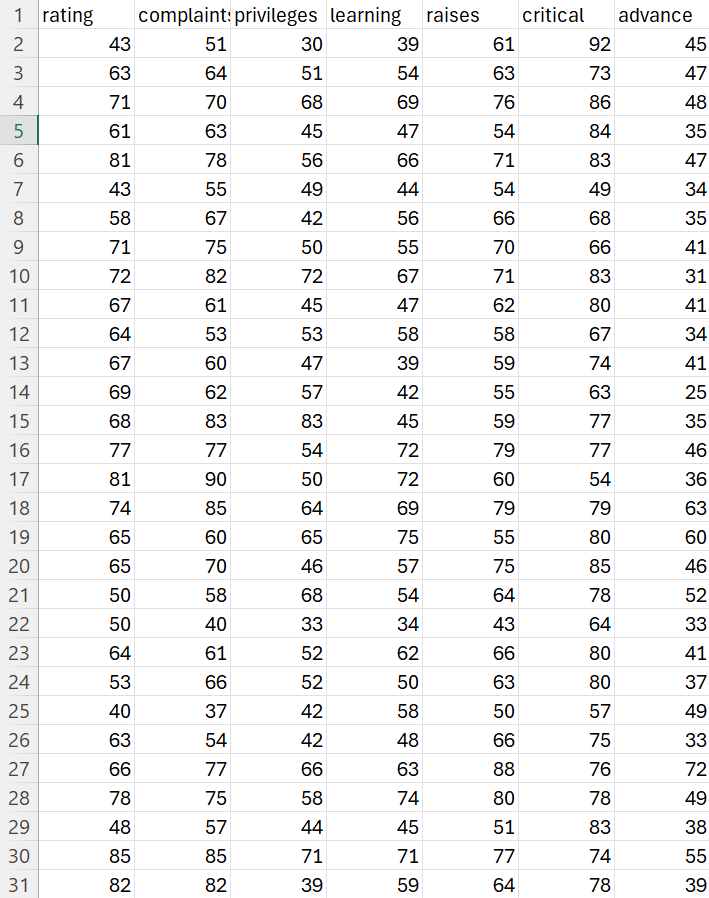
\includegraphics{./Excel_1_Unit/Week1_Diego/Week_1DJ/screenshots/Attitude_Base.png}

** Background Information **

\begin{itemize}
\tightlist
\item
  No context was given for the data set
\item
  7 columns: rating, complaint, privileges, leaning, raises, critical,
  advance
\item
  Rating attitude
\end{itemize}

\subsection{Filtering}\label{filtering}

(How to Follow) -Use Condition Formating (In Home) -Highlight cells,
equalt too or less than (58.5)

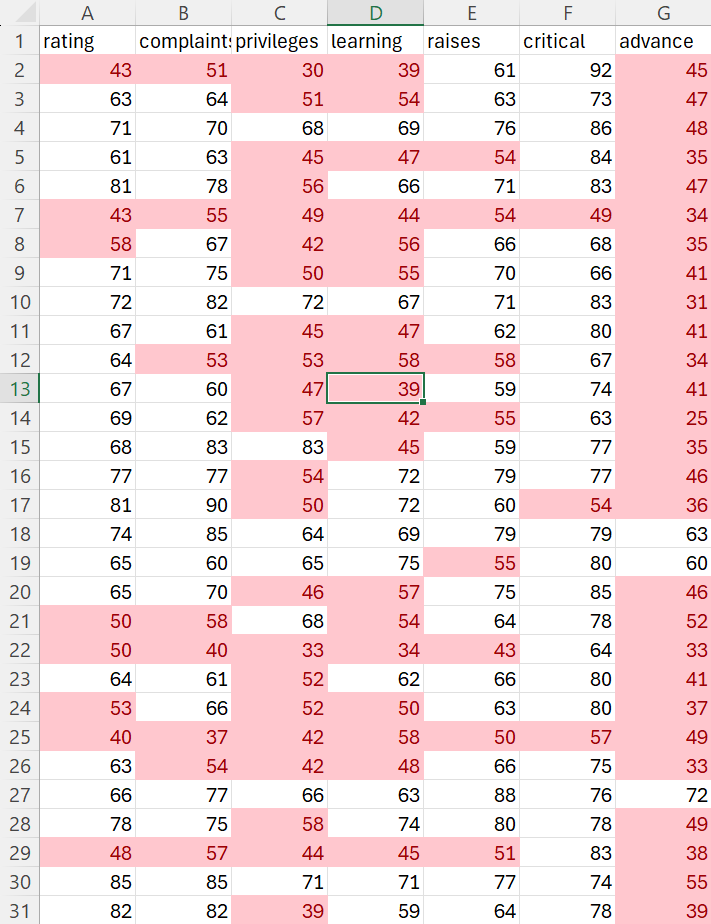
\includegraphics{./Excel_1_Unit/Week1_Diego/Week_1DJ/screenshots/Attitude_Base1.png}

\subsection{Observations}\label{observations}

-Each column has at least 2 cells =\textless50 -Advance attitude perform
poorly in an standard normal look(Bigger = Better) -Critical attitude
excelling in an standard normal look(Bigger = Better) -

\subsection{Filtering + Formulas}\label{filtering-formulas}

(How to Follow) -Select group of Cells, Rows or Columns -Use Condition
Formating (In Home) -Highlight cells, duplicate

-Select group of Cells, Rows or Columns -Select Formulas -Use Average,
Ma, Min

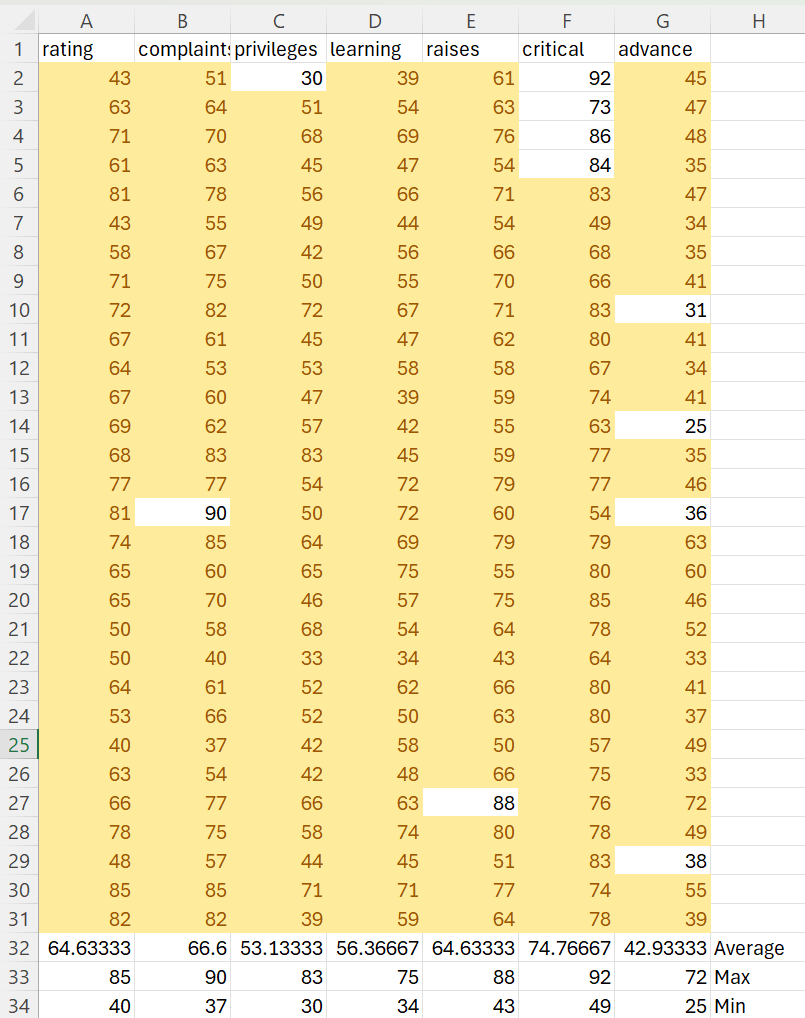
\includegraphics{./Excel_1_Unit/Week1_Diego/Week_1DJ/screenshots/Attitude_Base2.png}

\subsection{Observations}\label{observations-1}

\begin{itemize}
\tightlist
\item
  11 unique values that do not overlap/duplicated in another cell
\item
  Highest value was Critical with 92, Complaint had the 2nd highest with
  90, -\textgreater{} However that value appears to an outliar
\end{itemize}

-Minimum belongs to advance with 25 with privilege 2nd lowest with 30.
-Critical with the highest average with 74.77 complaint 2nd highest with
66.59

\subsection{Graphs}\label{graphs}

(How to Follow) -Select group of Cells, Rows or Columns -In the setting
insert, select graph or recommend graph

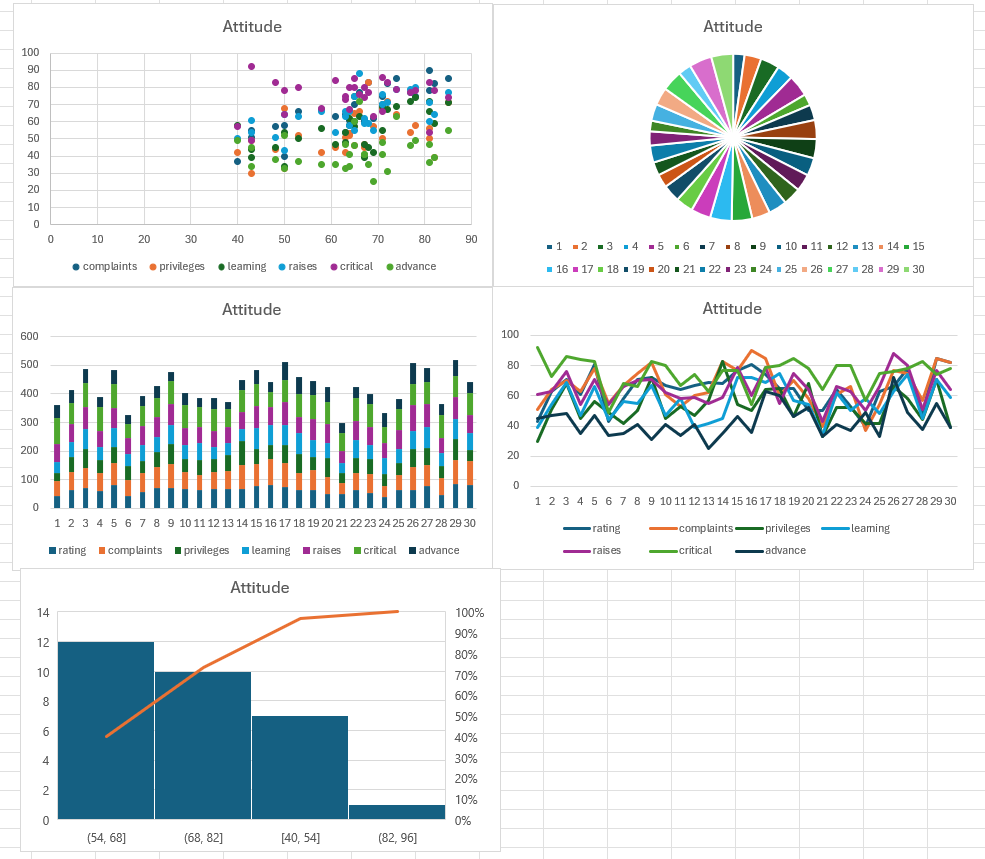
\includegraphics{./Excel_1_Unit/Week1_Diego/Week_1DJ/screenshots/Attitude_Base3.png}

\subsection{Observations}\label{observations-2}

\begin{itemize}
\tightlist
\item
  Bar graphs and pie graphs are not ver useful and do not provide any
  sort of information or trends
\end{itemize}

-The scatter plot is useful seeing where the cluster is and having a
visual provided of where those values are in relation to each other
-\textgreater Trends Complaints and learning has a postie correlation in
related to rating. The higher the rating the higher the complaint
attitude

-Statics chart helpful in showing where the concentration of the overall
data is.

-Best graph that represent the data was Scatter plot,
-\textgreater Easier to individual points and groups. -\textgreater Can
apply basic functions, or understanding to see trends -\textgreater{}
Overall seem that those with Combative attitudes excelled, those who
were humble seemed to a had a positive trend and privileged posh
attitudes performed worse than counterparts.

\subsection{Summary}\label{summary}

-Applied skills learned from Monday -Found trends patterns and made
conclusions -Researched possible data sets and other techniques

\section{Friday}\label{friday}

\subsection{Overview}\label{overview-1}

-Cleaning and filtering data in relation to soil samples -Applying
techniques learned from Monday and Wednesday to data set -Document all
necessary actions for repeatable research -Find a story in the data

\subsection{Data Information}\label{data-information}

-Data is from the USDA -Multiple different data sets that could be
chosen -\textgreater Friday's focuses on solid yield from 1984 - 1993
-Specific data can be found pressing the link
\href{https://agdatacommons.nal.usda.gov/articles/dataset/Data_from_Tillage_and_cropping_effects_on_soil_quality_indicators_in_the_northern_Great_Plains/26673769?file=48572716}{Data
from Tillage and cropping effects on soil quality indicators in the
northern Great Plains}

-The study provides insights into how soil properties respond to crop
rotation and tillage practices under rainfed conditions in a semiarid
continental climate

\subsubsection{Column Name and
Information}\label{column-name-and-information}

PLOT: Plot number, identifying the specific plot where the data was
collected. REP: Replicate number, indicating the repetition of the
experiment or sampling within the plot. ROTATION: Crop rotation system
used in the experiment, typically represented by a code. -TILLAGE:
Tillage treatment, also represented by a code (e.g., T1, T2). -DEPTH:
Soil sampling depth (in cm). -SBD: Soil bulk density (g/cm³). -EC:
Electrical conductivity (dS/m), a measure of soil salinity. -PH: Soil pH
level. -NO3N: Nitrate nitrogen (mg/kg), an indicator of soil nitrogen
content. -SOC: Soil organic carbon (mg/kg). -TN: Total nitrogen (mg/kg).
-PMN: Potentially mineralizable nitrogen (mg/kg). -POMLF: Particulate
organic matter light fraction (mg/kg). -POMSF: Particulate organic
matter small fraction (mg/kg). -POMT: Total particulate organic matter
(mg/kg). -POMSOM: Particulate organic matter as a percentage of soil
organic matter. -MBC: Microbial biomass carbon (mg/kg). -MBN: Microbial
biomass nitrogen (mg/kg)

\subsection{Intial Observation}\label{intial-observation}

(How to Follow) -Select group of Cells, Rows or Columns -Select column
with depth,(Step1) -select all 7.5cm (Step2) -shift arrow
-\textgreater{} 4 rows (Step3) -In the setting insert, select graph or
recommend graph(Step4) -For this we used a Column cluster(reccomended)

\subsubsection{7.5 cm depth}\label{cm-depth}

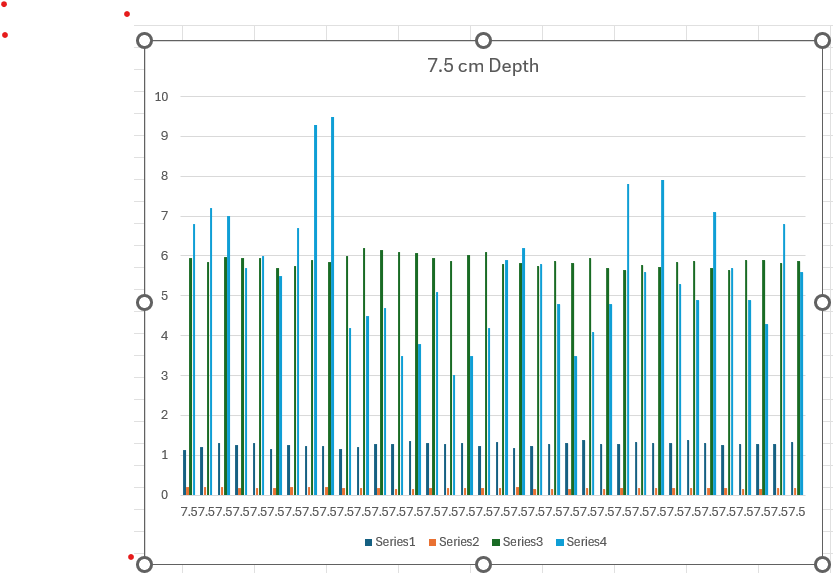
\includegraphics{./Excel_1_Unit/Week1_Diego/Week_1DJ/screenshots/Soil1.png}

\subsubsection{15 cm depth}\label{cm-depth-1}

-Repeats steps, changing 7.5 to 15

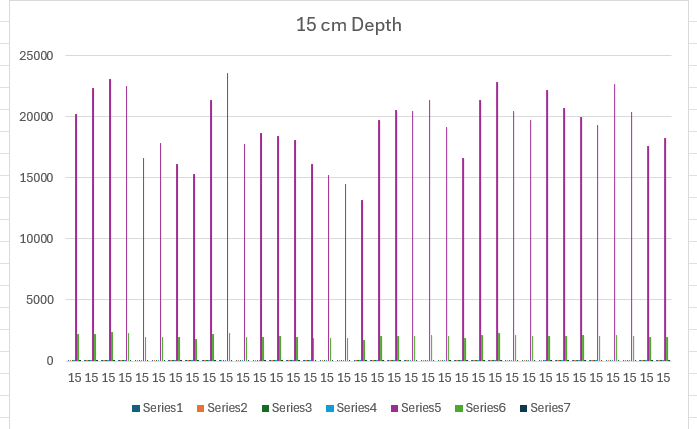
\includegraphics{./Excel_1_Unit/Week1_Diego/Week_1DJ/screenshots/Soil2.png}

\subsubsection{30 cm depth}\label{cm-depth-2}

-Repeats steps, changing 7.5 to 30

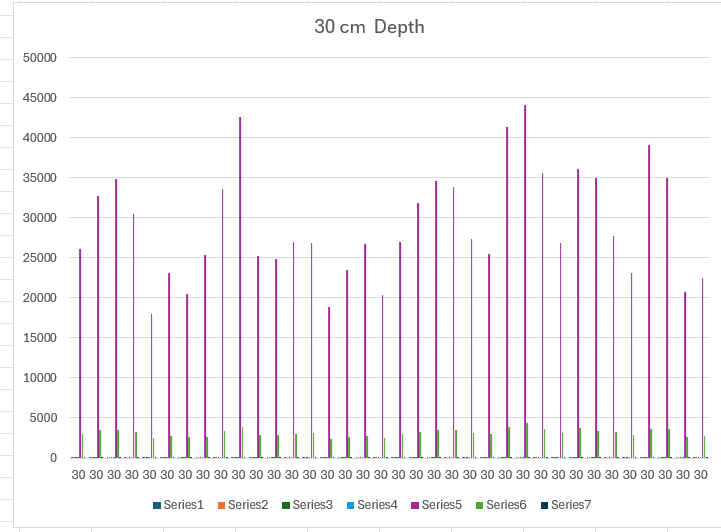
\includegraphics{./Excel_1_Unit/Week1_Diego/Week_1DJ/screenshots/Soil3.png}

\subsection{observations}\label{observations-3}

-On Graphs 2 \& 3 seem to lacking a series 4 and both have high series 7
-On Graph 1 lacks series 5-7 and series

\subsection{Focus + 2nd graph}\label{focus-2nd-graph}

-Focused on 2 columns ph and NO3N -\textgreater PH level and nitrogen.

-Highlighted each PH and NO3N for each respective depth -Selected graphs
for each a line graph

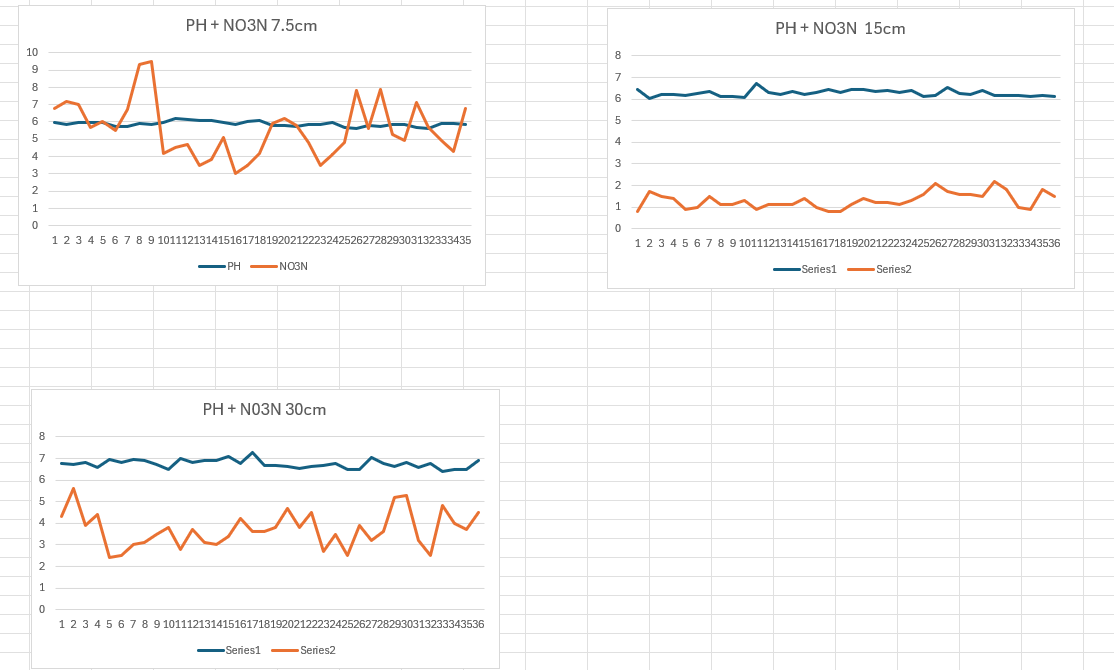
\includegraphics{./Excel_1_Unit/Week1_Diego/Week_1DJ/screenshots/Soil4.png}

\subsubsection{Observations}\label{observations-4}

-Depth seems to correlate to steadier levels in PH and N03N to 15cm
-15cm depth seems to the best to hold consistent level in PH and N03N
-7.5cm depth has the largest variance highest Max in NO3n -30cm depth
had the lowest valley in NO3N

\subsection{Formatting}\label{formatting}

-Highlight cells rule, less than value (6.25) -Highlighted each PH and
NO3N for each respective depth

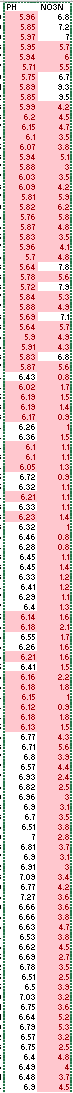
\includegraphics{./Excel_1_Unit/Week1_Diego/Week_1DJ/screenshots/Soil5.png}
\#\#\#\# Observations

-30 + 15 cm depths' nitrogen is below 6.25 cm -7.5cm depth's PH is below
6.25

\subsection{Summary}\label{summary-1}

-Worked with team lead and Professor at data sets and possible ideas
-Discussed what expectations were set and what documentation should look
like -Worked on USDA data set -Applied skills and tools to dataset

\subsection{Notes for next work}\label{notes-for-next-work}

-Larger and more background information on a dataset is useful -Lacked
comparsion test to 1984 data set -Extended research into subject
provides a working platform -Large data sets become complicated to work
with and see at once on excel

\bookmarksetup{startatroot}

\chapter{NASA Earth Data - Samuel
Zelaya}\label{nasa-earth-data---samuel-zelaya}

\section{Week 1 - 08/28/2024}\label{week-1---08282024}

\subsection{Wednesday}\label{wednesday-1}

\subsubsection{Recap and Quarto Document
Guidance}\label{recap-and-quarto-document-guidance}

\textbf{Activity:} The class began with a more in-depth explanation of
Quarto documents for those unfamiliar with the process.

\textbf{Topics Covered:}

1.Naming and building Quarto notes.

2.Professor V. used a student example to create a small Excel sheet
based on the student's daily food intake and corresponding calorie
count.

3.He built a graph of the food items and their calorie counts, then
demonstrated how to insert the graph into a Quarto document.

4.Provided guidance on how to log the information effectively within
Quarto to meet his expectations.

\subsubsection{Practical Application: Excel Data
Visualization}\label{practical-application-excel-data-visualization}

\textbf{Activity:} Continued from Monday's class.

\textbf{1.Task:} Repeated the data cleaning and visualization process
with a different dataset.

\textbf{2.Dataset Used:} Economics dataset.

\textbf{3.Data Preparation:} - Checked for NA values or empty cells
(none were found). - Sorted the data in ascending order based on date
values. - Focused on the relationship between \texttt{psavert} (personal
savings rate) and \texttt{uempmed} (median duration of unemployment).

\subsubsection{Data Visualization
Process}\label{data-visualization-process}

\textbf{1.Graphs Created: I} Created a line , bar graphs and scatter
plot, to find which ne was the easiest to interpreted to explore the
relationship between \texttt{psavert} and \texttt{uempmed} from
different perspectives.

\textbf{2.Final Choice:} I selected scatter plot graph, the line bar
graph i found it unclear how to interpret the scatter plot provided a
clearer and easier-to-read visualization of the data.

\textbf{3.Additional Observations:}

There are a few points where the personal saving rate is relatively low.
This might indicate special circumstances or different economic
conditions during those periods. The two variables don't seem to have a
strong linear relationship. The points are fairly scattered, indicating
that changes in the personal saving rate don't consistently correlate
with changes in the median duration of unemployment.

\subsubsection{Key Takeaways from Professor
V.}\label{key-takeaways-from-professor-v.}

\textbf{Understanding Context:}

\begin{enumerate}
\def\labelenumi{\arabic{enumi}.}
\item
  It's crucial to understand the context of your dataset before deciding
  on the type of visualization.
\item
  Once the dataset is understood, choose visualizations that effectively
  compare relationships between columns (e.g., petal length vs.~petal
  width in another example; in this case, \texttt{psavert}
  vs.~\texttt{uempmed}).
\end{enumerate}

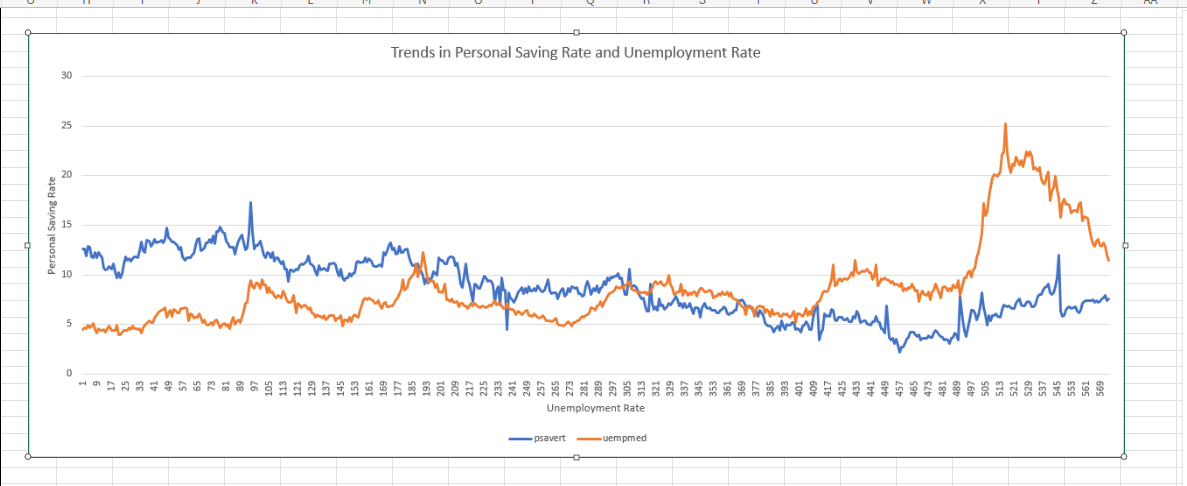
\includegraphics{./Excel_1_Unit/Week1_Samuel/Screenshot(355).png}

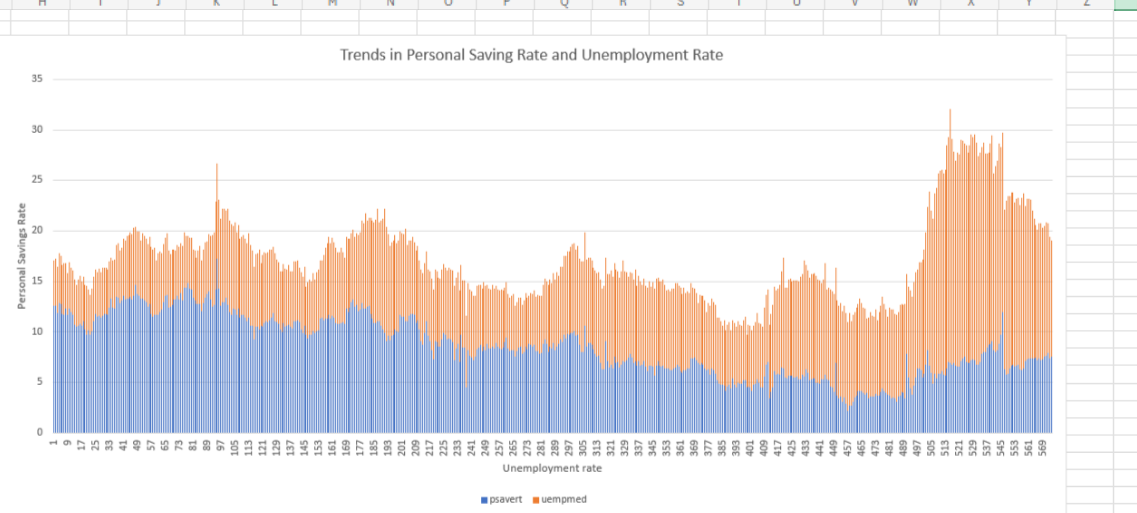
\includegraphics{./Excel_1_Unit/Week1_Samuel/Screenshot(356).png}

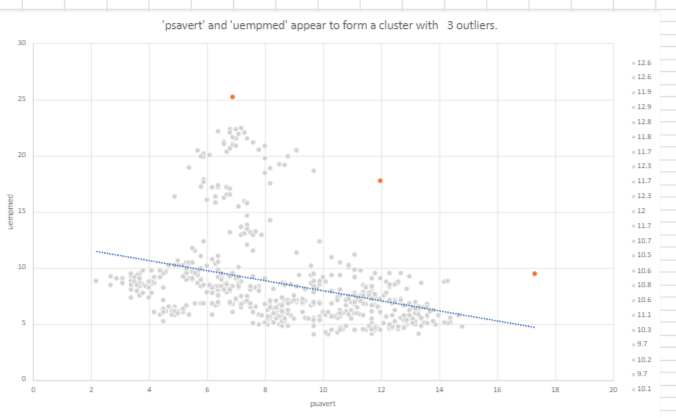
\includegraphics{./Excel_1_Unit/Week1_Samuel/Screenshot(360).png}

\begin{center}\rule{0.5\linewidth}{0.5pt}\end{center}

\subsection{Friday}\label{friday-1}

\subsubsection{Class Activity}\label{class-activity}

Today, we worked in class with our groups, focusing on our individual
datasets. I chose to work with NASA Earth Data, a resource I'll be
utilizing throughout the semester.

\subsubsection{Dataset Exploration}\label{dataset-exploration}

I began by exploring the \href{https://www.earthdata.nasa.gov/}{NASA
Earth Data} portal, which offers a broad range of datasets across
various topics like the atmosphere, earth quality, biosphere, human
dimensions, and sun-earth interactions. Each main topic is further
divided into subtopics, where users can download data in formats like
CSV and Excel.

The portal also features a ``Learn'' section that provides tutorials and
guides on how to read and use the data particularly useful for those new
to the platform.

\subsubsection{Dataset Selection}\label{dataset-selection}

I was particularly interested in the ``Human Dimensions'' topic, which
explores how humans interact with Earth's resources. After filtering the
available datasets by format (CSV and Excel) and sorting by the oldest
end date, I selected the dataset titled \textbf{Effects of Climate
Change on Global Food Production from SRES Emissions and Socioeconomic
Scenarios}.

This dataset caught my attention because global food production has
always been of interest to me, especially considering the drastic
changes in soil quality and agricultural methods over the years.
Additionally, the way human activities have affected the soil and food
production varies significantly by country.

\subsubsection{Dataset Overview}\label{dataset-overview}

\emph{Climate Change and Global Food Production}

\textbf{Summary:}

The agricultural sector is facing significant challenges due to
population growth, land degradation, and urbanization, all of which
threaten global food production. Climate change is expected to intensiy
these challenges, particularly in regions vulnerable to drought and
famine.

A NASA study used crop modeling to assess the impacts of climate change
on food production. The study emphasizes that water availability and
temperature are critical factors affecting crop yields. It also
considers the effects of CO2 and suggests that climate change could have
a significant impact on global food production, prices, and the risk of
hunger.

\subsubsection{Data Analysis}\label{data-analysis}

\begin{enumerate}
\def\labelenumi{\arabic{enumi}.}
\item
  I downloaded the dataset and opened it in Excel to begin the data
  cleaning process. The dataset covers average crop production for
  various countries from 2000-2006. For this analysis, I focused on the
  variables: country code, wheat, rice, maize, and added a new variable
  for the year. I first calculated the mean, maximum, and minimum
  production values for each country for wheat, rice, and maize. China
  had the highest production values across all three variables---wheat,
  rice, and maize. On the other hand, Venezuela had the lowest
  production for wheat, Saudi Arabia for rice, and Japan for maize. To
  visualize this, I created a 100\% stacked column chart. The graph
  shows that maize is the most produced crop across all countries, while
  wheat and rice exhibit irregular consistency over the years from 2000
  to 2006.
  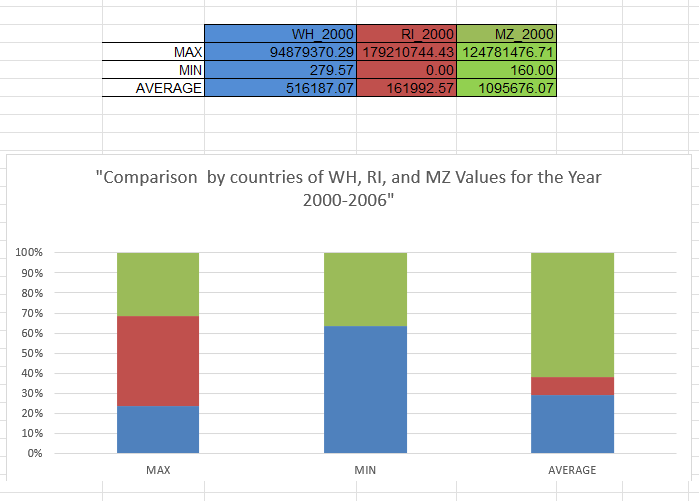
\includegraphics{./Excel_1_Unit/Week1_Samuel/Screenshot (372).png}
\item
  Next, I created a pie chart to confirm my hypothesis. The chart
  reveals that maize has the highest average production among the three
  crops, suggesting it might be more widely cultivated or more important
  in global agriculture compared to wheat and rice. Rice also has a
  relatively high average production, indicating its global importance
  as a staple food. Wheat, despite having the lowest average production
  among the three, still shows a substantial
  amount.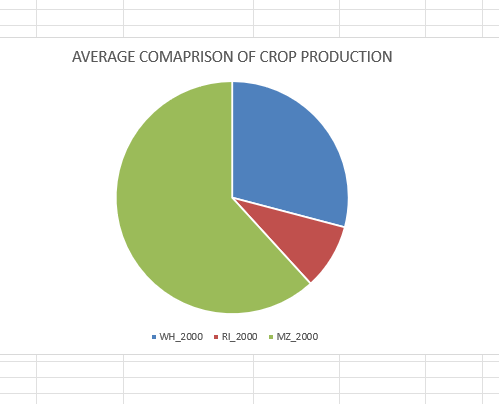
\includegraphics{./Excel_1_Unit/Week1_Samuel/Screenshot(373).png}
\item
  . Additionally, I created another stacked column chart to view the
  crop production across all 74 countries. This broader analysis
  revealed that China has the highest production numbers, while
  Switzerland has the lowest. I calculated the average production for
  each crop for each country and determined the maximum and minimum
  average production across the three crops for each country. The
  results show Switzerland with the lowest average production overall,
  and India with the second highest average production, as reflected in
  the
  graph.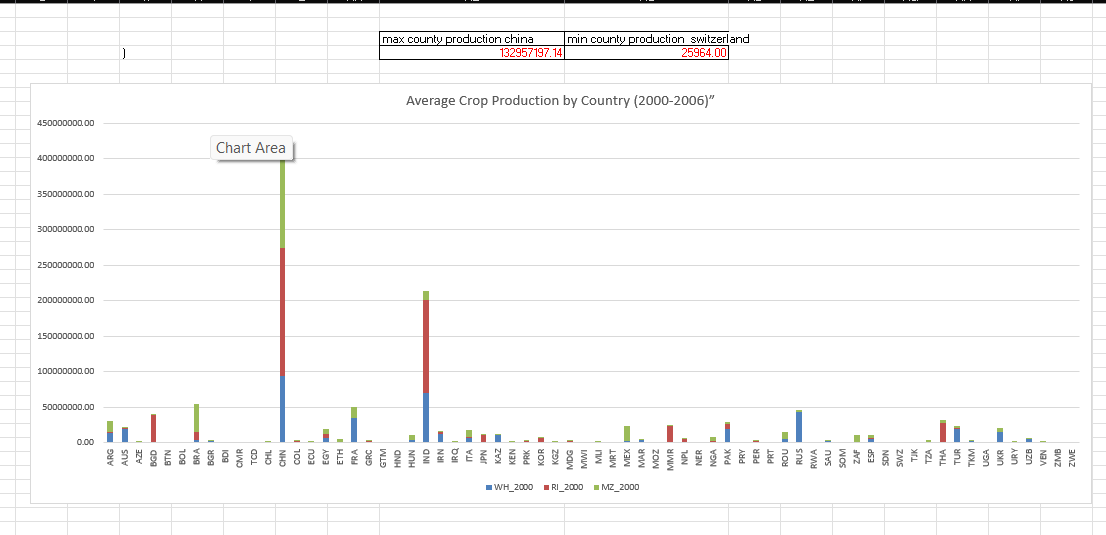
\includegraphics{./Excel_1_Unit/Week1_Samuel/Screenshot(374).png}
\item
  In the scatter plot, I observed a strong relationship between the
  production of wheat and rice. China and India were identified as clear
  outliers with extremely high production values for all crops. This
  plot helps in visualizing the tendencies and relationships between the
  production levels of different crops across
  countries.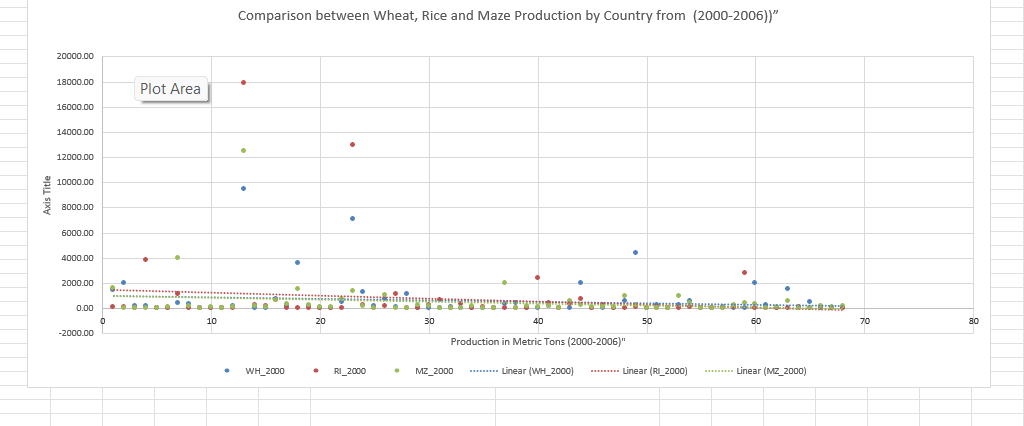
\includegraphics{./Excel_1_Unit/Week1_Samuel/Screenshot(375).png}
\item
  Then created a line graph to analyze production trends over time.
  Although China and India have the highest production points, the chart
  reveals a lack of consistency in their production levels. In contrast,
  wheat and maize, while showing lower production values, exhibit more
  consistent levels across countries. Nations with consistently low
  production lines may face agricultural challenges or have less focus
  on these
  crops.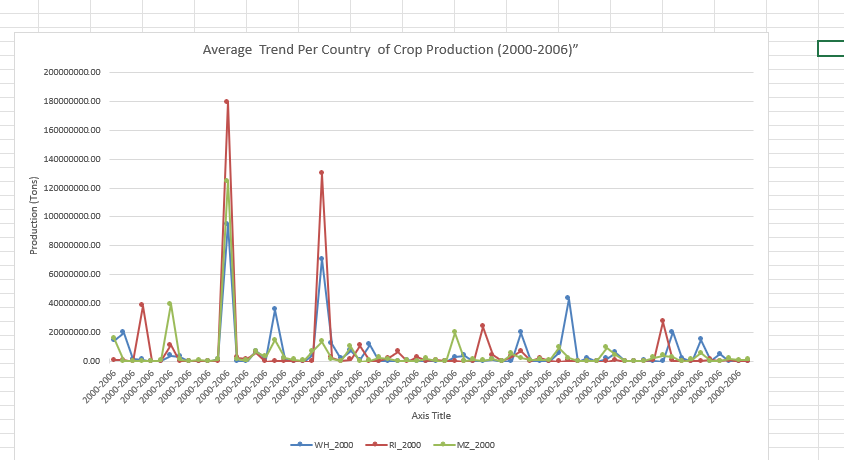
\includegraphics{./Excel_1_Unit/Week1_Samuel/Screenshot(376).png}
\end{enumerate}

\subsubsection{Summarize insights}\label{summarize-insights}

\begin{enumerate}
\def\labelenumi{\arabic{enumi}.}
\item
  China (CHN) leads in production with the highest values across all
  crops---wheat, rice, and maize---showing significant output in each
  category.
\item
  Switzerland (SW) exhibits the lowest production values across all
  crops, indicating minimal agricultural output.
\item
  China has the highest average production per country, reflecting its
  extensive agricultural operations and capacity.
\item
  Countries with low average production, such as Switzerland and
  Swaziland, highlight their limited agricultural activities and output.
\item
  Maize has the highest maximum production values across several
  countries, underscoring its significant role in global agriculture.
\item
  Rice shows high production values in several countries, including
  China and India, emphasizing its importance as a staple food.
\item
  Wheat production is relatively high in several countries but is not as
  dominant as maize or rice.
\end{enumerate}

\bookmarksetup{startatroot}

\chapter{Federal Reserve Economic Data - Janice
Oenardi}\label{federal-reserve-economic-data---janice-oenardi}

\section{Wednesday}\label{wednesday-2}

\subsection{Cleaning the dataset}\label{cleaning-the-dataset}

Before processing and creating visualizations of the dataset, it is
important to prep the dataset by cleaning it. There might be N/A values
or outliers in the dataset, which needs to be removed and cleaned to
create better and more accurate visualizations.

To clean the data, there are a few things that can be done: - Finding
and highlighting NA values by selecting the range of cells and doing
`Conditional Formatting' to `Highlight Cells Rules'. - Removing NA
values by using the `Find and Replace'. Find `NA' and replace it with
`0'. - Using IF function to check for NA values and replace it
accordingly. Ex: =IF(A2=``NA'', ``0'', A2)

Additionally, upon converting the Swiss dataset from a .csv format into
an Excel, the first column of the dataset became combined into one cell.

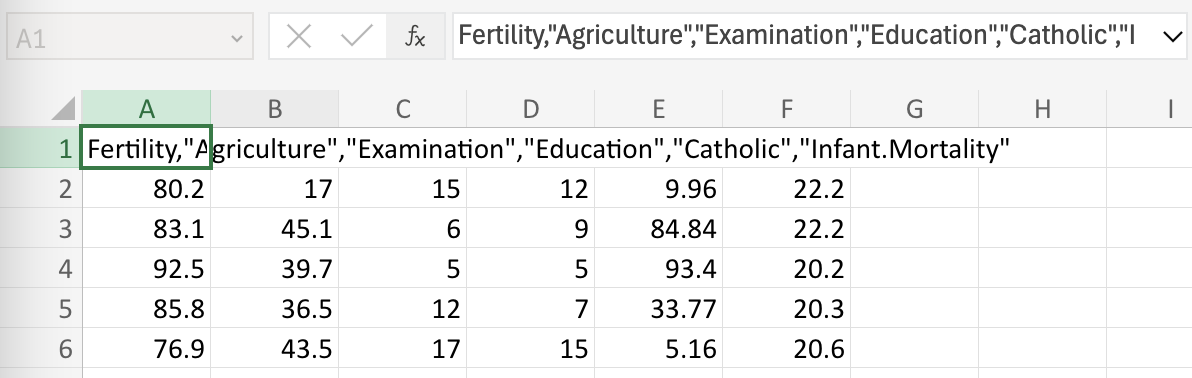
\includegraphics{./Excel_1_Unit/Week1_Janice/Week 1/Week 1 Wednesday/Swiss_cleaning.png}

I fixed the titles that are separated by commas in the one cell by
separating the titles into the different respective columns.

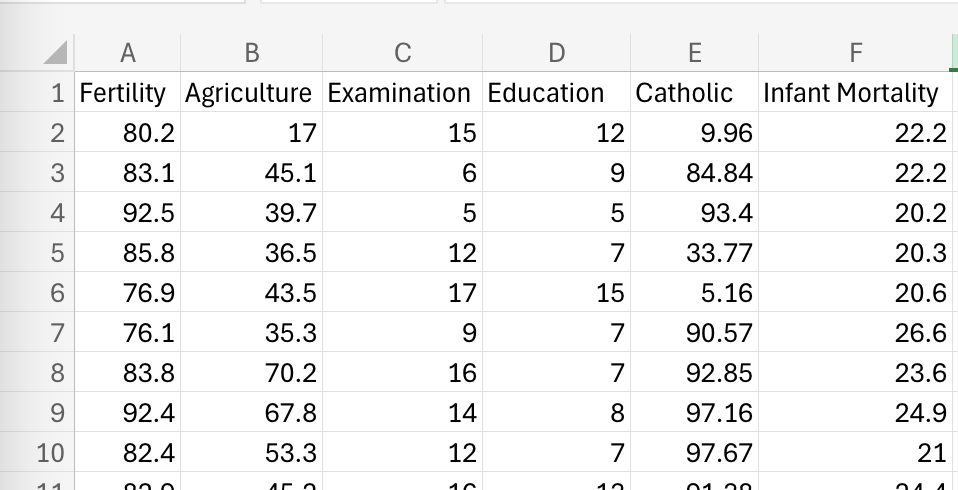
\includegraphics{./Excel_1_Unit/Week1_Janice/Week 1/Week 1 Wednesday/Swiss_cleaning2.png}

\subsection{Context of dataset}\label{context-of-dataset}

Before creating plots and visualizations of the dataset, it is important
to know what each title in the columns mead and understand the context
of the dataset.

\url{https://stat.ethz.ch/R-manual/R-patched/library/datasets/html/swiss.html}

The dataset contains 47 French-speaking ``provinces'' in Switzerland at
around 1888. During that year, Switzerland was entering a demographic
transition, where its fertility rates was beginning to fall from the
typical level of underdeveloped countries. There are 6 variables in the
dataset, where variables are scaled from 0 to 100, except Cathloic that
is scaled from 0 to 1. The definitions of the dataset are as below:

\begin{itemize}
\tightlist
\item
  Fertility = common standardized fertility measure
\item
  Agriculture = \% of males involved in agriculture as occupation
\item
  Examination = \% draftees receiving highest mark on army examination
\item
  Education = \% education beyond primary school for draftees.
\item
  Catholic = \% `catholic' (as opposed to `protestant').
\item
  Infant.Mortality = live births who live less than 1 year.
\end{itemize}

\subsection{Creating Different Basic
Visualizations}\label{creating-different-basic-visualizations}

\subsubsection{Scatterplot 1 - Fertility and Cathlic appear to cluster
in two groups with four
outliers}\label{scatterplot-1---fertility-and-cathlic-appear-to-cluster-in-two-groups-with-four-outliers}

In creating plots, I utilized Excel's tool of Recommended Charts, which
included a scatterplot of `Fertility' and `Catholic'. The scatterplot
shown below shows two groups of cluster with four outliers.

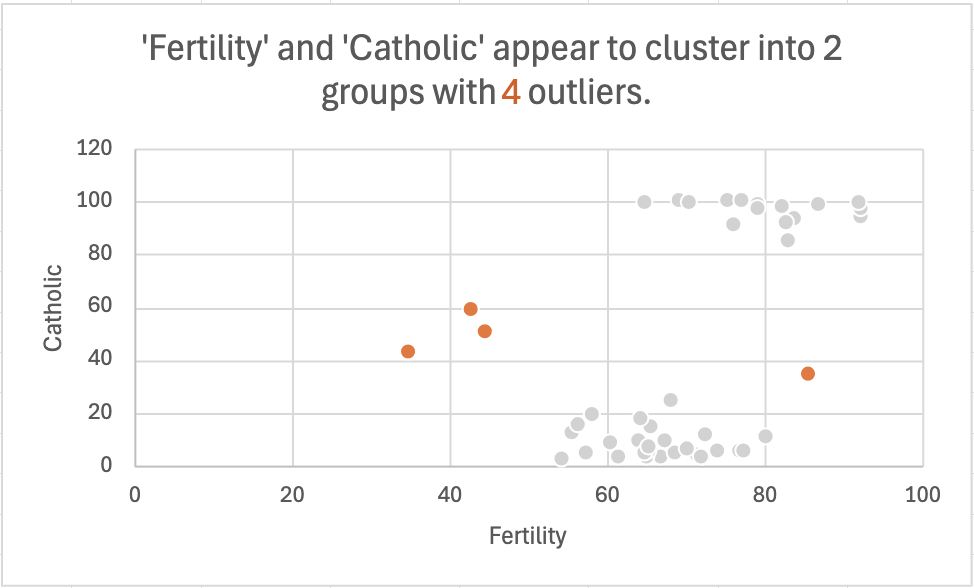
\includegraphics{./Excel_1_Unit/Week1_Janice/Week 1/Week 1 Wednesday/Swiss_scatterplot.png}

As shown in the scatterplot, provinces with higher percentage of
Catholic people seem to have a slightly higher fertility compared to
provinces with low percentage of Catholic people.

\subsubsection{Scatterplot 2 - Relationship between infant mortality and
percentage of Catholic people in a
province}\label{scatterplot-2---relationship-between-infant-mortality-and-percentage-of-catholic-people-in-a-province}

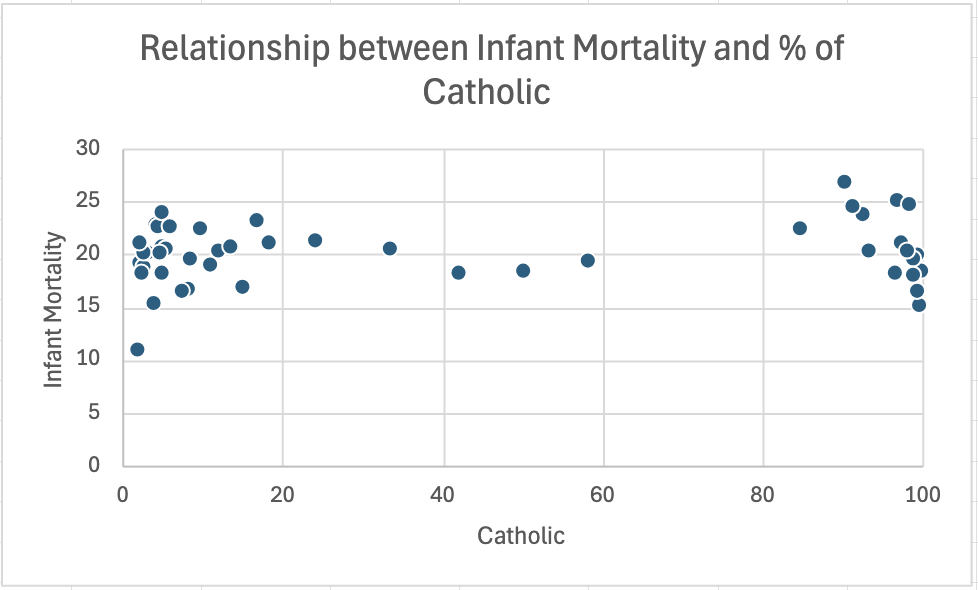
\includegraphics{./Excel_1_Unit/Week1_Janice/Week 1/Week 1 Wednesday/Swiss_scatterplot2.png}
Based on the scatterplot above, infant mortality and Catholic appear to
have no apparent relationship. However, provinces with higher percentage
of Catholic population appear to has a slightly higher infant mortality,
with a few provinces having 25 and more live births in a year.
Meanwhile, the provinces with a low percentage of Catholic population
appear to have infant mortality mostly in the 15-25 range.

Aside from that, the provinces in Swiss appear to have either a very
high percentage of Catholic population or a very low percentage of
Catholic population, with the scatterplot showing two clusters on the
lower end of Catholic percentage (0-20\%) and a higher end of Catholic
percentage (80-100\%). What do you observe?

\subsubsection{Bar Charts}\label{bar-charts}

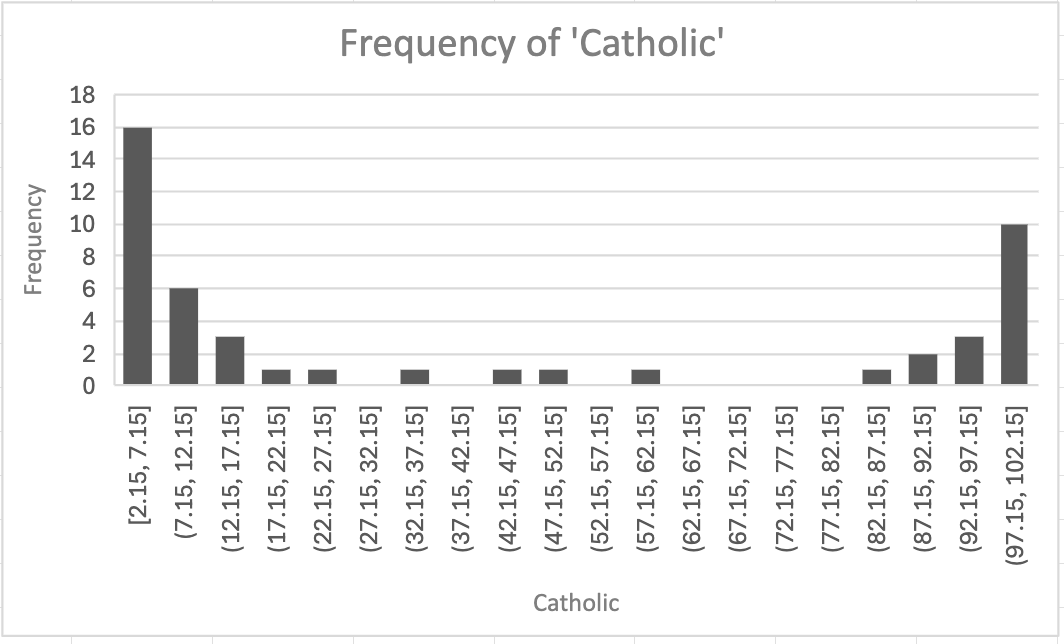
\includegraphics{./Excel_1_Unit/Week1_Janice/Week 1/Week 1 Wednesday/Swiss_barchart.png}
As mentioned in the discussion above, the provinces in Swiss appear to
have either a very high percentage of Catholic population, or a very low
percentage of Catholic population. The bar chart shows a high frequency
within the 2.15-7.15\% of Catholic population that gradually decreases
as the percentage approaches 17.15-22.15 and gradually increases again
as it approaches the 87.15-92.15 percentage of Catholic population. The
bar chart above better visualize the two groups of highly populated
Catholic province or lowly populated Catholic province.

\subsubsection{Line Chart}\label{line-chart}

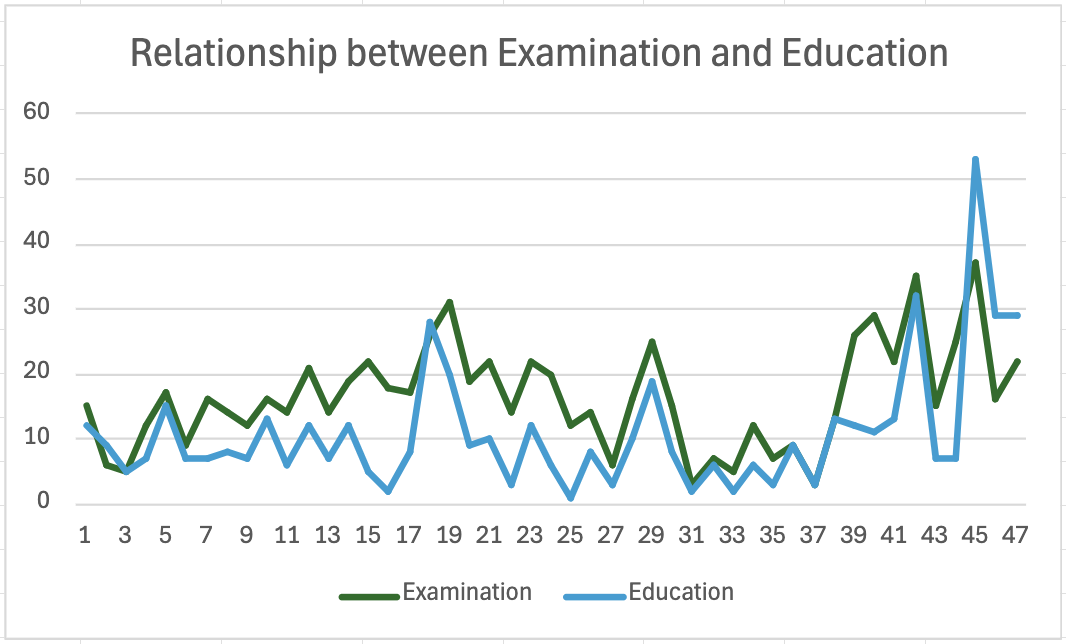
\includegraphics{./Excel_1_Unit/Week1_Janice/Week 1/Week 1 Wednesday/Swiss_linechart.png}
The line chart above clearly shows that there is a direct relationship
between examination and education. As the percentage of education beyond
primary school for draftees increases, the percentage of draftees
receiving highest mark on army examination also increases. The two
variables showcase a positive directly correlated relationship. Aside
from that, the graph also shows that the 46th province outperformed all
of the other provinces with the highest percentage of education beyond
primary school for draftees and also the highest percentage of draftees
receiving highest mark on army examination. The 46th province is
followed by the 42th province which has the second highest percentage of
education beyond primary school and second highest percentage of
draftees receiving highest mark on army examination.

\subsubsection{Pie Charts}\label{pie-charts}

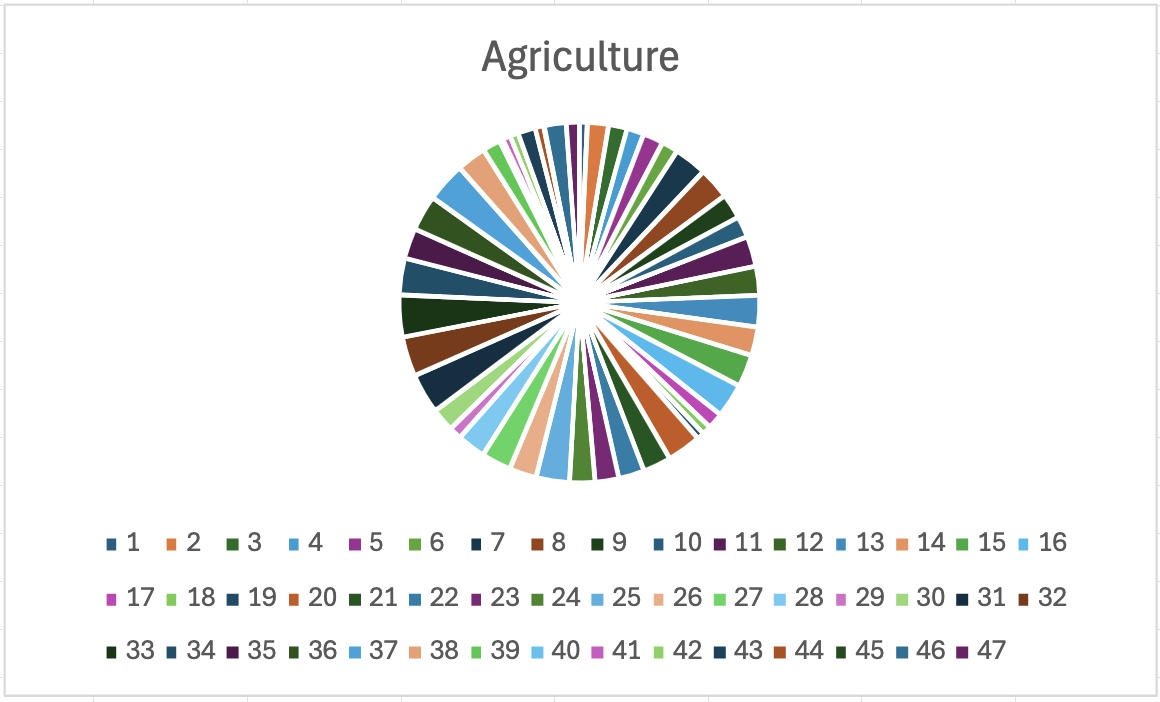
\includegraphics{./Excel_1_Unit/Week1_Janice/Week 1/Week 1 Wednesday/Swiss_piechart.png}
The pie chart does not really visualize the agriculture data well, as
there are too many percentage classification of males involved in
agriculture occupation. However, the pie chart can be made better by
making the classifications into 5 groups to see which range of
percentage of males involved in agriculture occupation is higher among
the other provinces.

\subsubsection{Histograms}\label{histograms}

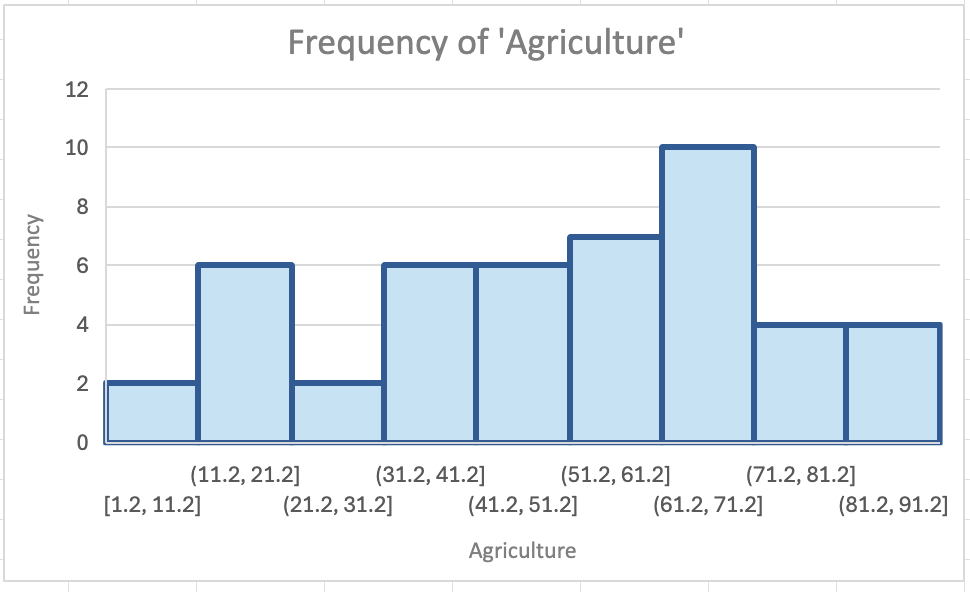
\includegraphics{./Excel_1_Unit/Week1_Janice/Week 1/Week 1 Wednesday/Swiss_histogram.png}
The histogram shows a slightly negative skew on the frequency of males
involved in agriculture as occupation. The majority of the provinces
have males involved in agriculture on the 61.2-71.2\% range. The
1.2-11.2\% range and the 21.2-31.2\% range of males involved in
agriculture have the lowest frequency.

\subsection{What plot represent better the data?
why?}\label{what-plot-represent-better-the-data-why}

There isn't any plot that is more superior that the other, but it wholly
depends on the variables being plotted. For instance, the relationship
between examination and education can be better represented using a line
chart, as a line chart shows a more visible distinction between the
variable of examination and education. If using a scatterplot, the many
plots in the chart may cause the distinction between the two variables
to be less visible, as the two variables are directly correlated and
have values very closely to one another.

On the other hand, using a scatterplot can better highlight the two
groups of highly-populated Catholic provinces and lowly-populated
Catholic provinces better than a barchart. The scatterplot can visualize
the two groups of clusters on opposite ends, highlighting there there
are two major groups in the Swiss: Catholic heavily-populated province
or Protestant heavily-populated province

Therefore,different plots have different uses and can highlight the
relationship of some variables better than the other, depending on the
context and relationship of the variables being plotted. It is important
to explore the different relationships of variables using different
charts and plots to better visualize the relationships of the variables
in the dataset.

\section{Friday}\label{friday-2}

\subsection{Choosing the source and
dataset}\label{choosing-the-source-and-dataset}

\begin{itemize}
\tightlist
\item
  The source that I chose for this class is the Federal Reserve Economic
  Data (FRED), with the link: \url{https://fred.stlouisfed.org/}.
\end{itemize}

I chose the FRED source because I would like to delve more into the US
economy to conduct economic analysis and financial research as a
business major. Additionally, there are a lot of different datasets,
including from different countries, that I an explore from the source.

\begin{itemize}
\tightlist
\item
  For this assignment, I used ChatGPT to brainstorm on which dataset I
  should choose from and why.
\end{itemize}

After using ChatGPT and exploring the source website some more, I
decided to choose the dataset containing Corporate Profits by Industry
with this link:
\url{https://fredaccount.stlouisfed.org/public/datalist/6257}. I
downloaded the whole data lists, as it all involves the relevant
corporate profits of different industries and sub-sectors.

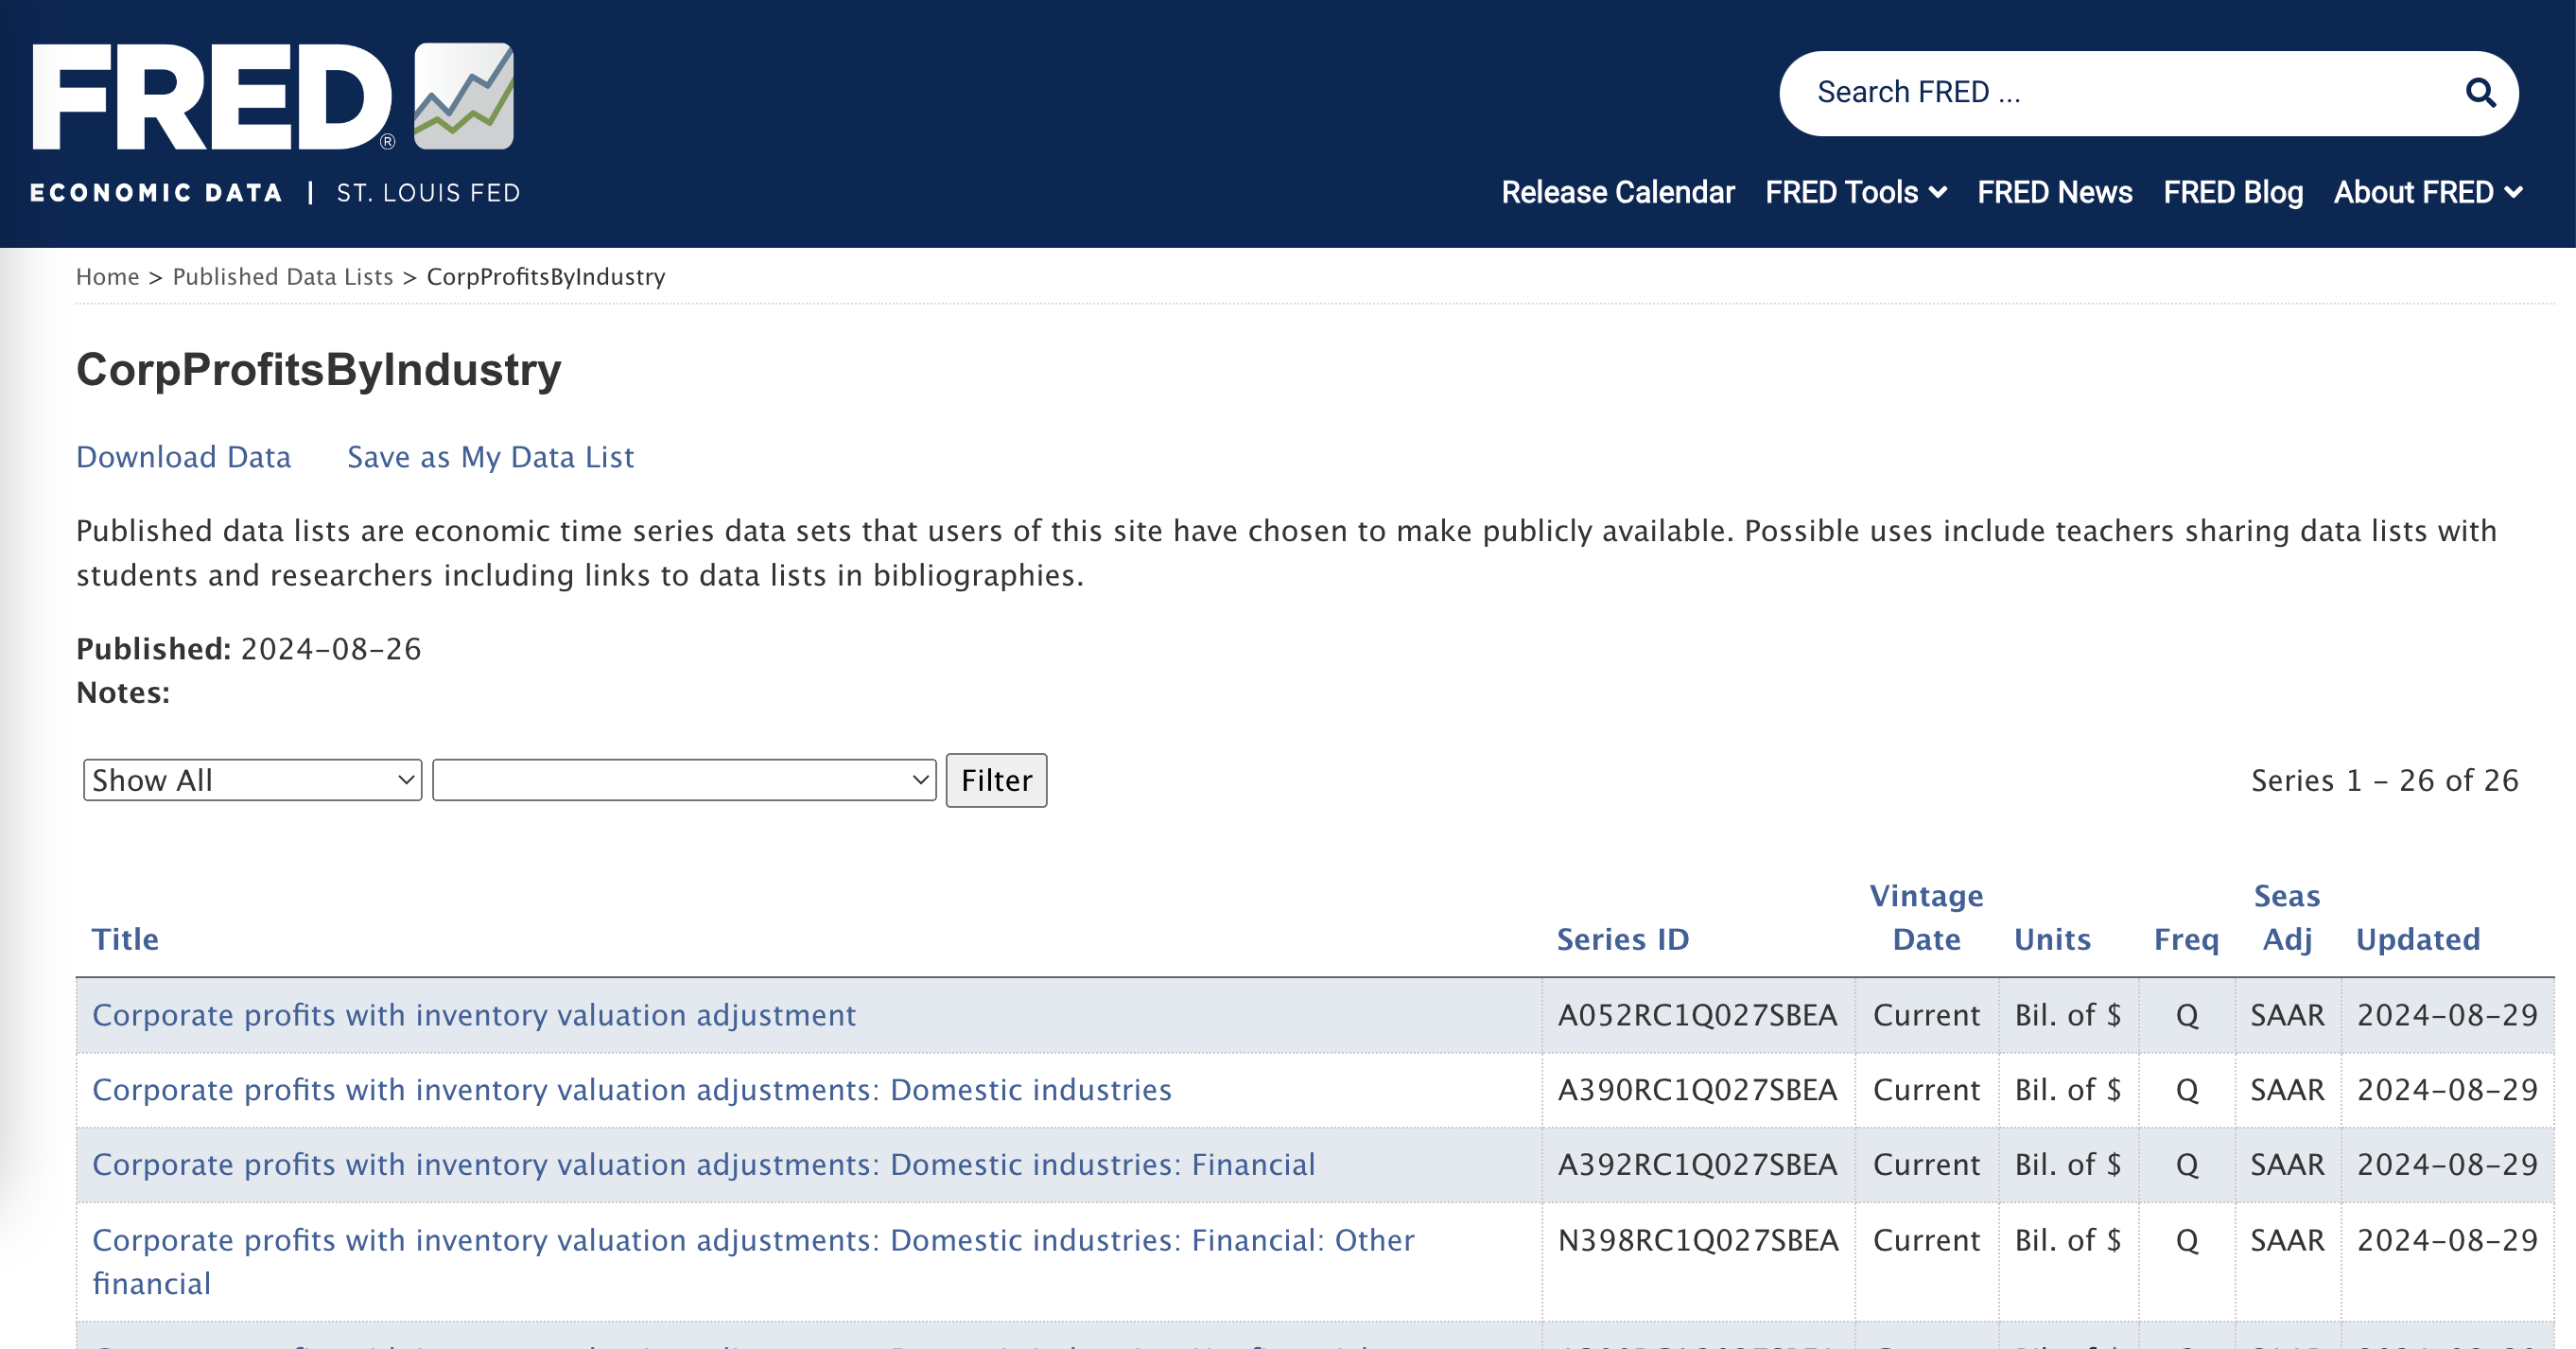
\includegraphics{./Excel_1_Unit/Week1_Janice/Week 1/Week 1 Friday/Download_data.png}

\begin{itemize}
\tightlist
\item
  I think that it would be interesting to visualize how the different
  industries' profits vary throughout the years, and whether there are
  correlations between any industries. I downloaded the dataset as Excel
  format.
\end{itemize}

\subsection{Context of the dataset}\label{context-of-the-dataset}

The dataset contains quarterly data on the corporate profits with
inventory valuation adjustment for different industries, including
non-financial, financial, federal, and many other sub-categories such as
manufacturing, wholesale trade, and utilities. The data is presented in
billions of dollars, seasonally adjusted annual rate. To set parameter,
the study for this assignment only looks at the 10 year span from first
quarter of 2014 to the first quarter of 2024.

\subsection{Cleaning and organizing the
dataset}\label{cleaning-and-organizing-the-dataset}

\begin{enumerate}
\def\labelenumi{\arabic{enumi}.}
\tightlist
\item
  Replacing Series ID with Titles
\end{enumerate}

The dataset contains columns with Series ID instead of titles.
Therefore, it needs to be replaced with the titles, which can be viewed
in the other sheet in the same Excel document. - To do this, I copied
the first Series ID and paste it on the `Find' tool.

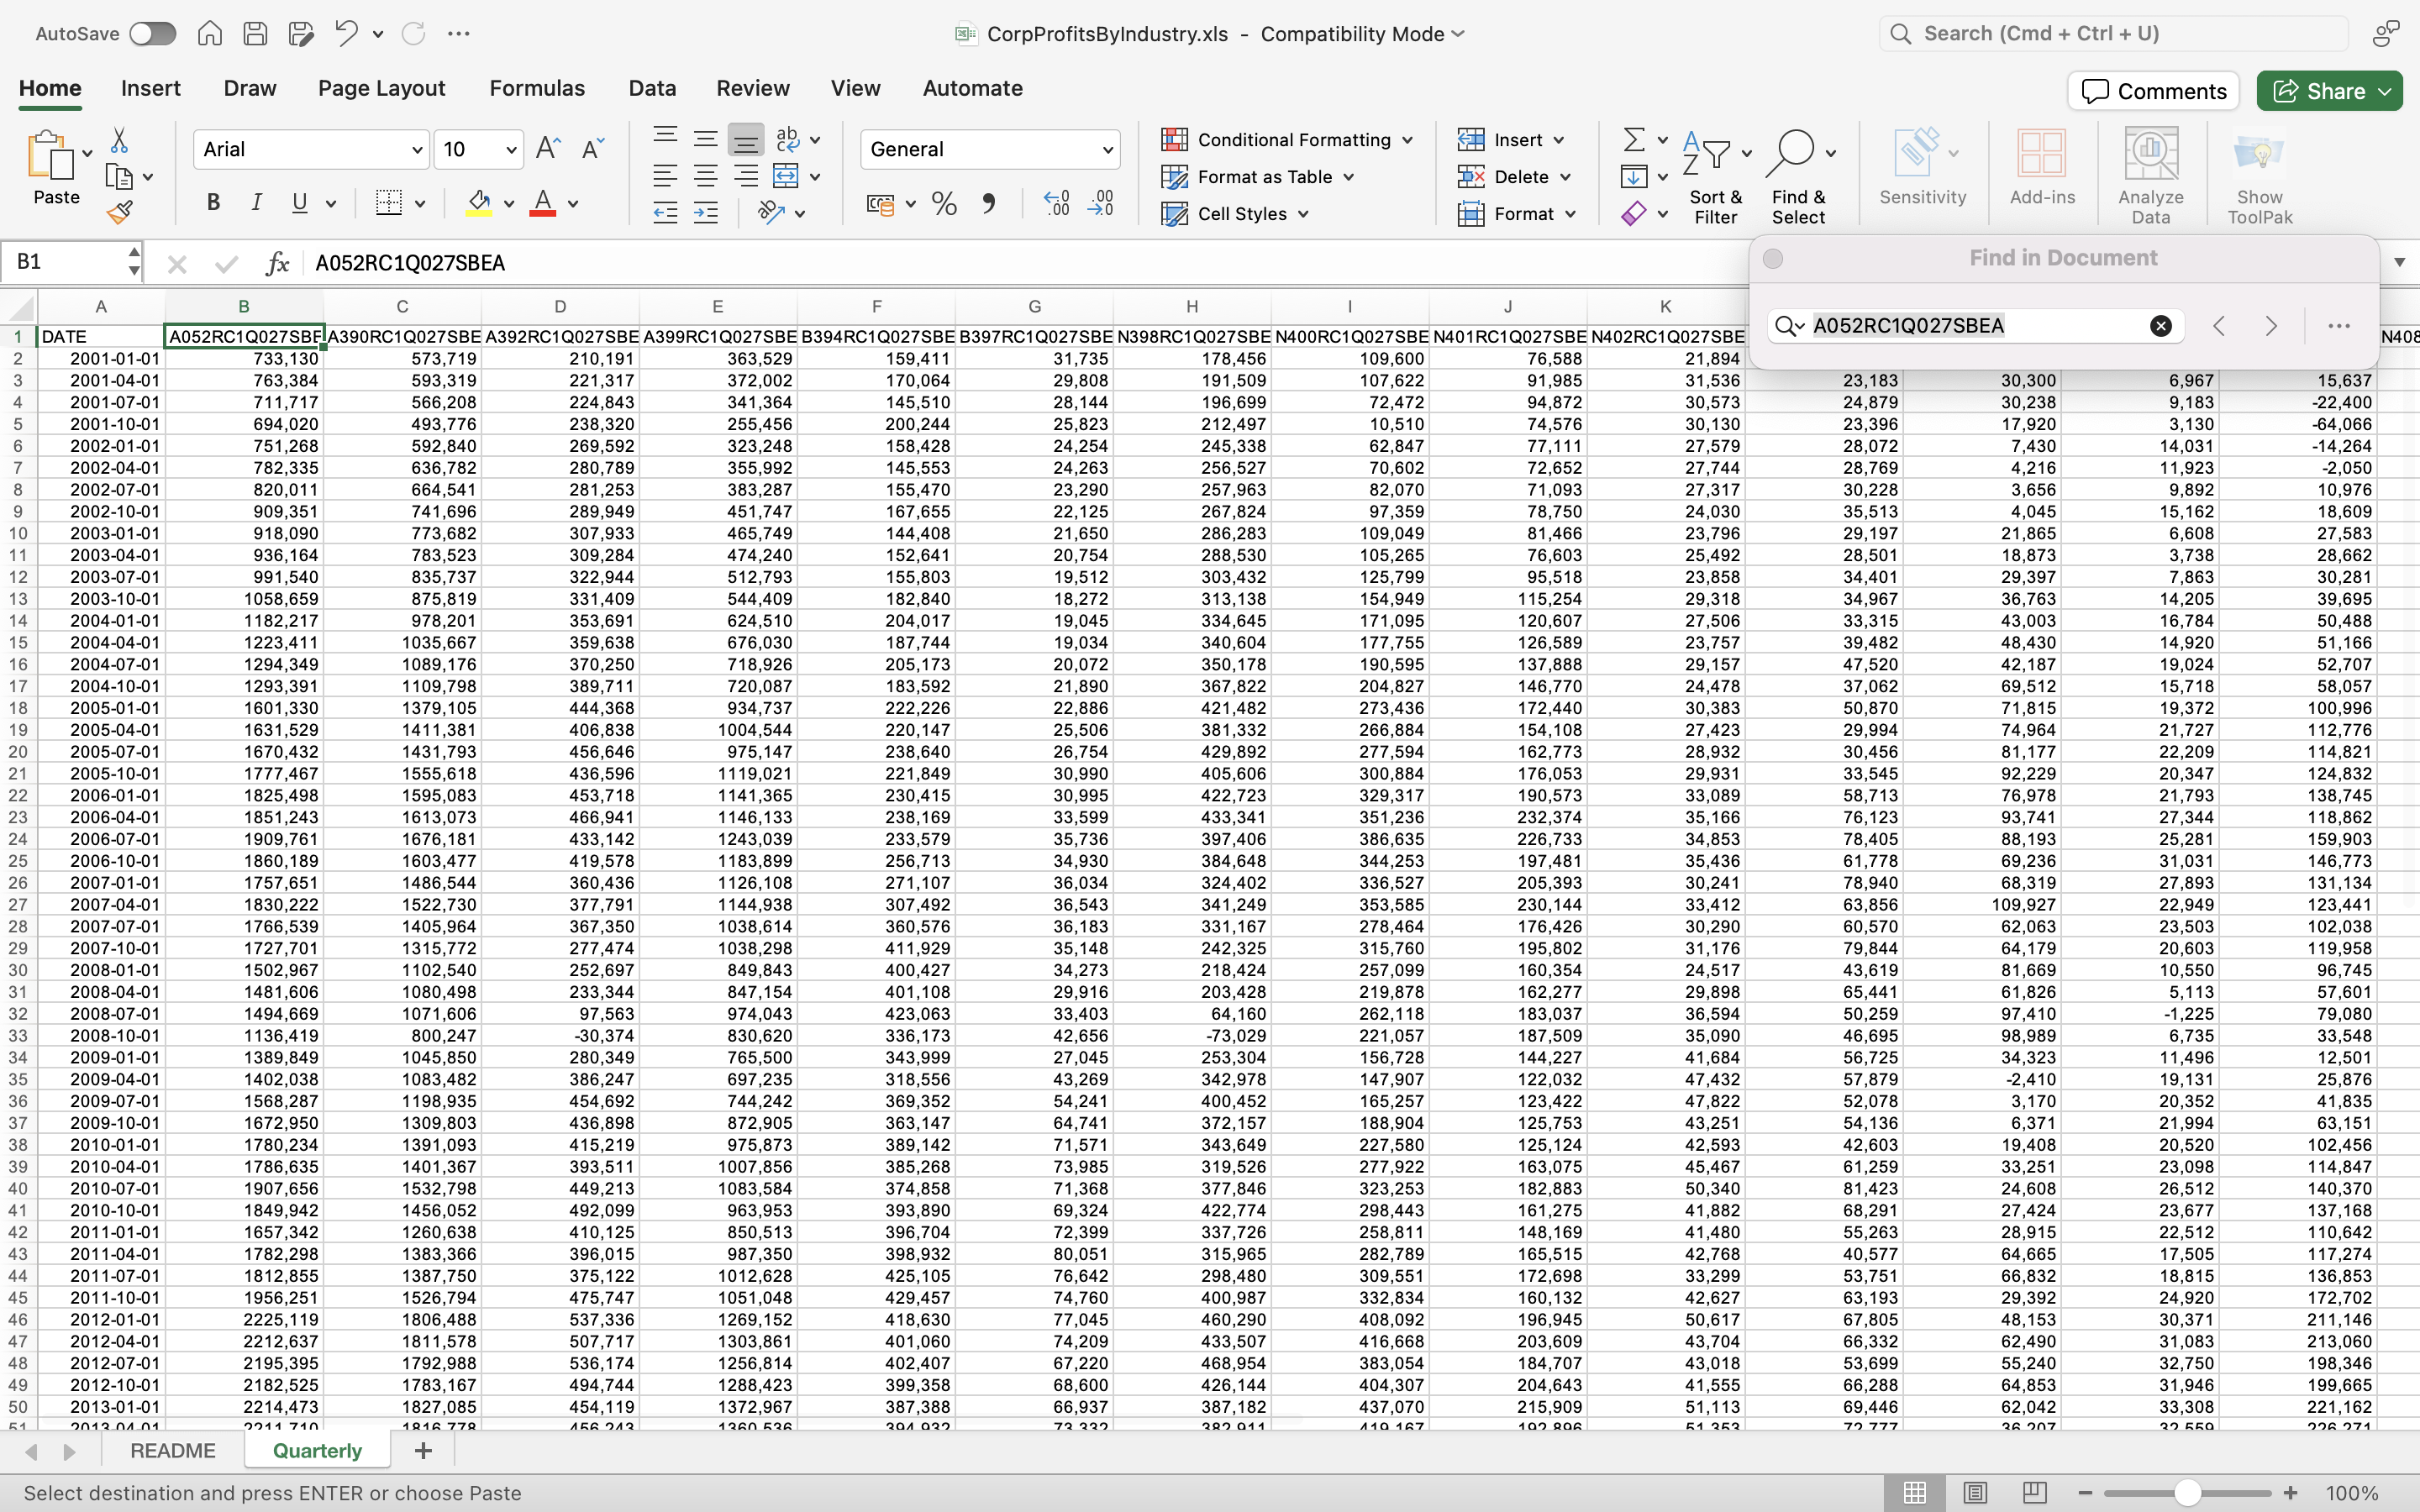
\includegraphics{./Excel_1_Unit/Week1_Janice/Week 1/Week 1 Friday/Replacing_column_titles.png}

\begin{itemize}
\tightlist
\item
  Then, I go to the other sheet in the same Excel document to find the
  same Series ID and locate the title
\end{itemize}

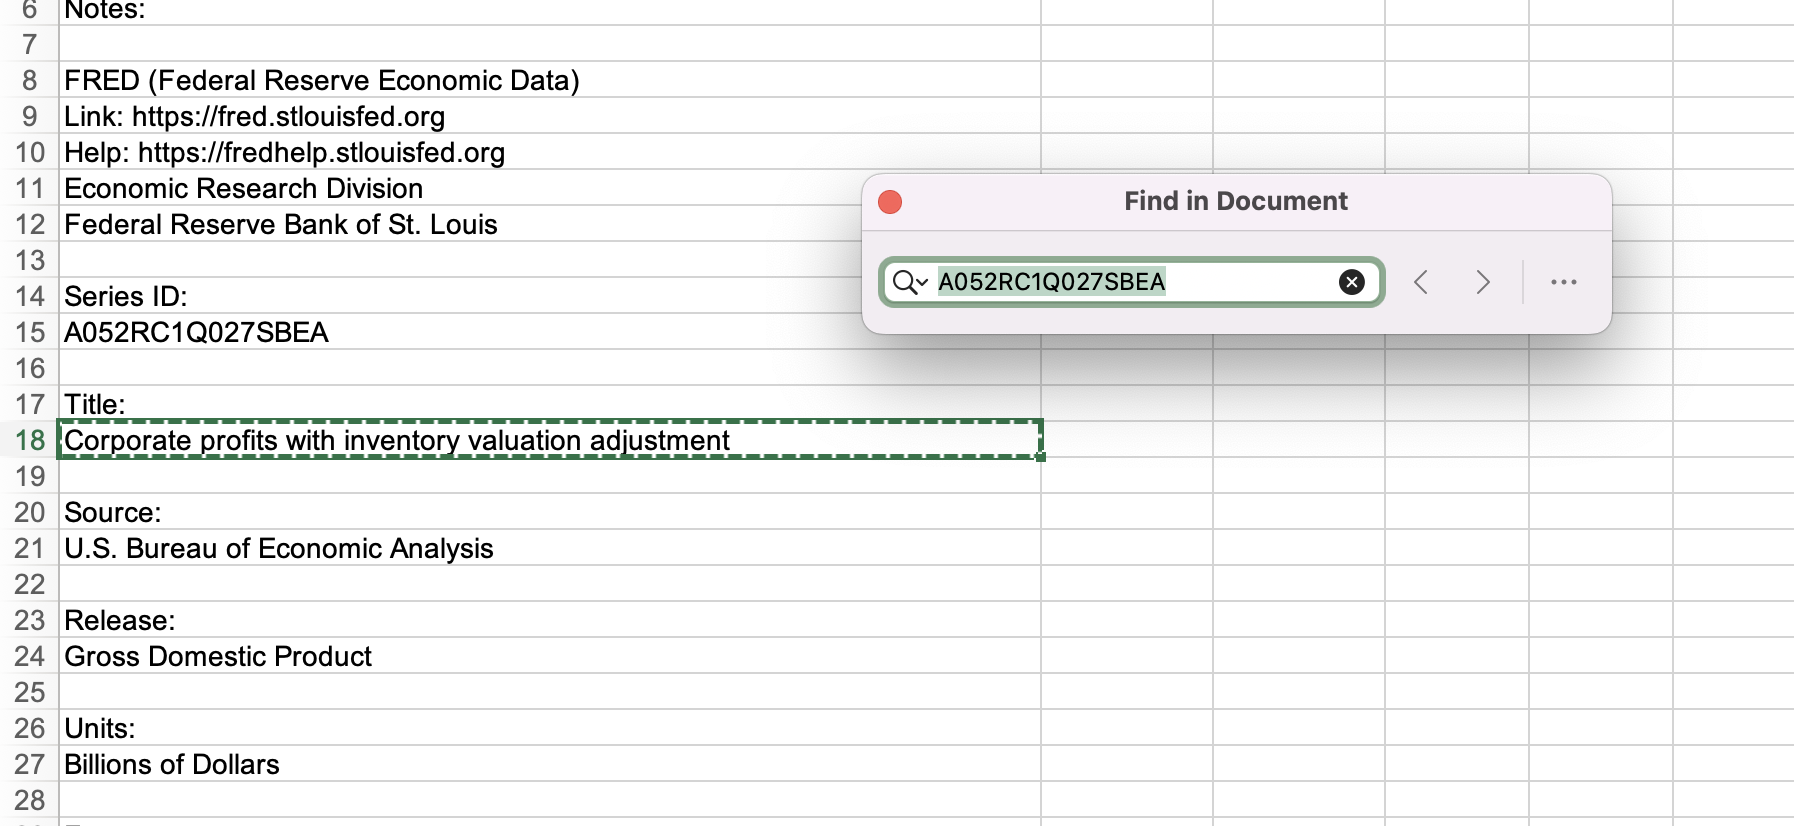
\includegraphics{./Excel_1_Unit/Week1_Janice/Week 1/Week 1 Friday/Replacing_column_titles2.png}

\begin{itemize}
\tightlist
\item
  After locating the title, I copied it and paste it on the dataset
  sheet to replace the Series ID with the right title.
\end{itemize}

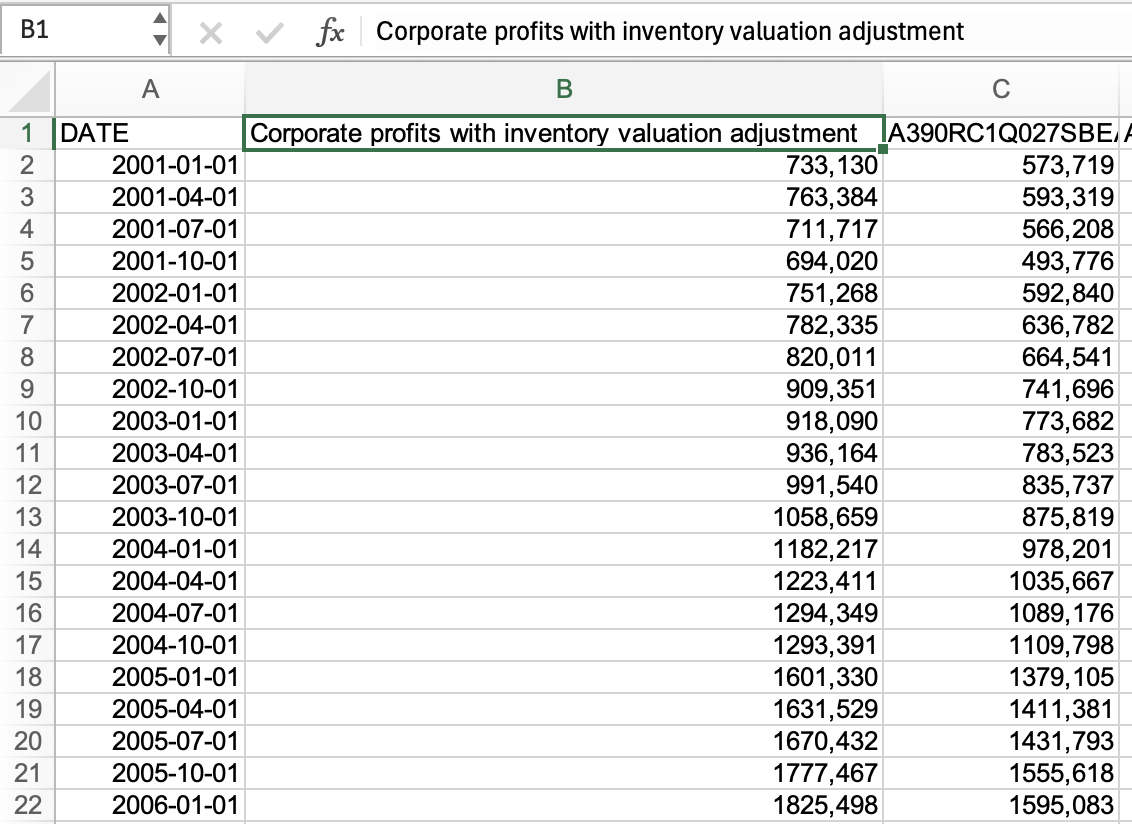
\includegraphics{./Excel_1_Unit/Week1_Janice/Week 1/Week 1 Friday/Replacing_column_titles3.png}

\begin{itemize}
\tightlist
\item
  Repeat this until all other Series ID are replaced with its title
\end{itemize}

\begin{enumerate}
\def\labelenumi{\arabic{enumi}.}
\setcounter{enumi}{1}
\item
  Making the titles more concise When copy and pasting back the titles
  to the dataset sheet, I realized that the titles are very long and
  repetitive. Therefore, I reorganized the title and make it shorter and
  more concise.
\item
  Formatting the columns to be more organized and neat To do this, I
  expanded the columns to the right width, and centered the text.
  Additionally, I also deleted the rows with data outside of the 10 year
  span from 2014 to 2024, as it is outside the parameter of the this
  exploration.
\end{enumerate}

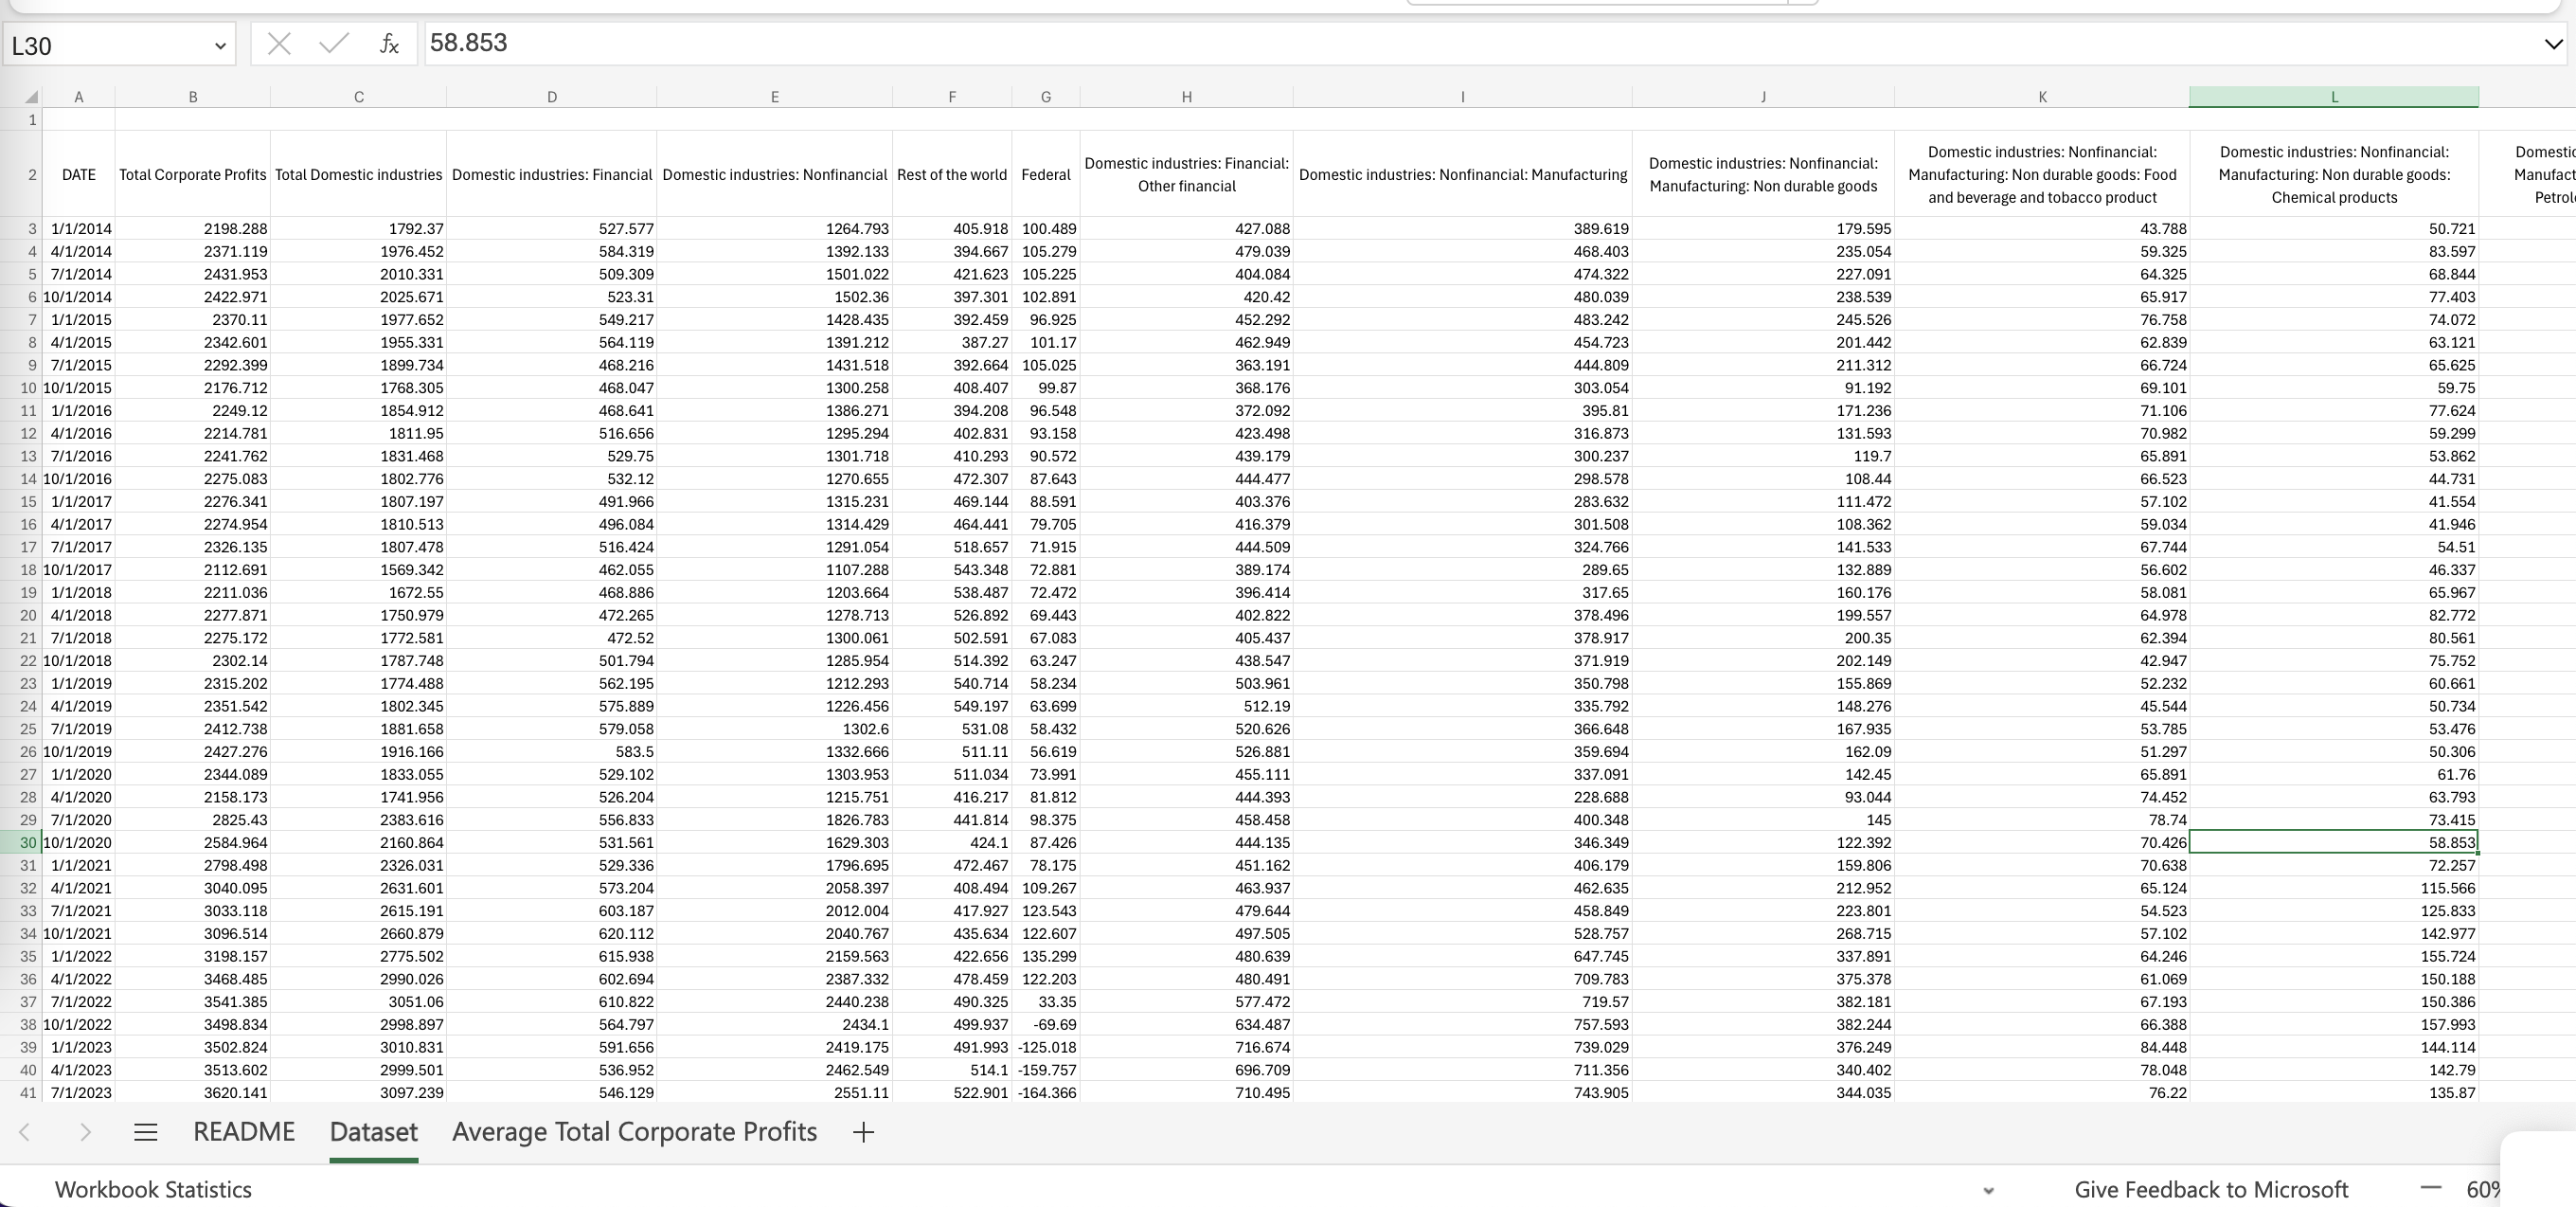
\includegraphics{./Excel_1_Unit/Week1_Janice/Week 1/Week 1 Friday/Cleaned_and_organized_data.png}

\subsection{Making Visualizations}\label{making-visualizations}

In making visualizations, I utilized Excel's `Recommended Charts' tool
under `Insert'. After using the tool, I looked over the data and explore
to create more meaningful visualizations on my own.

\subsubsection{Line chart: Average Total Profits in 10
Years}\label{line-chart-average-total-profits-in-10-years}

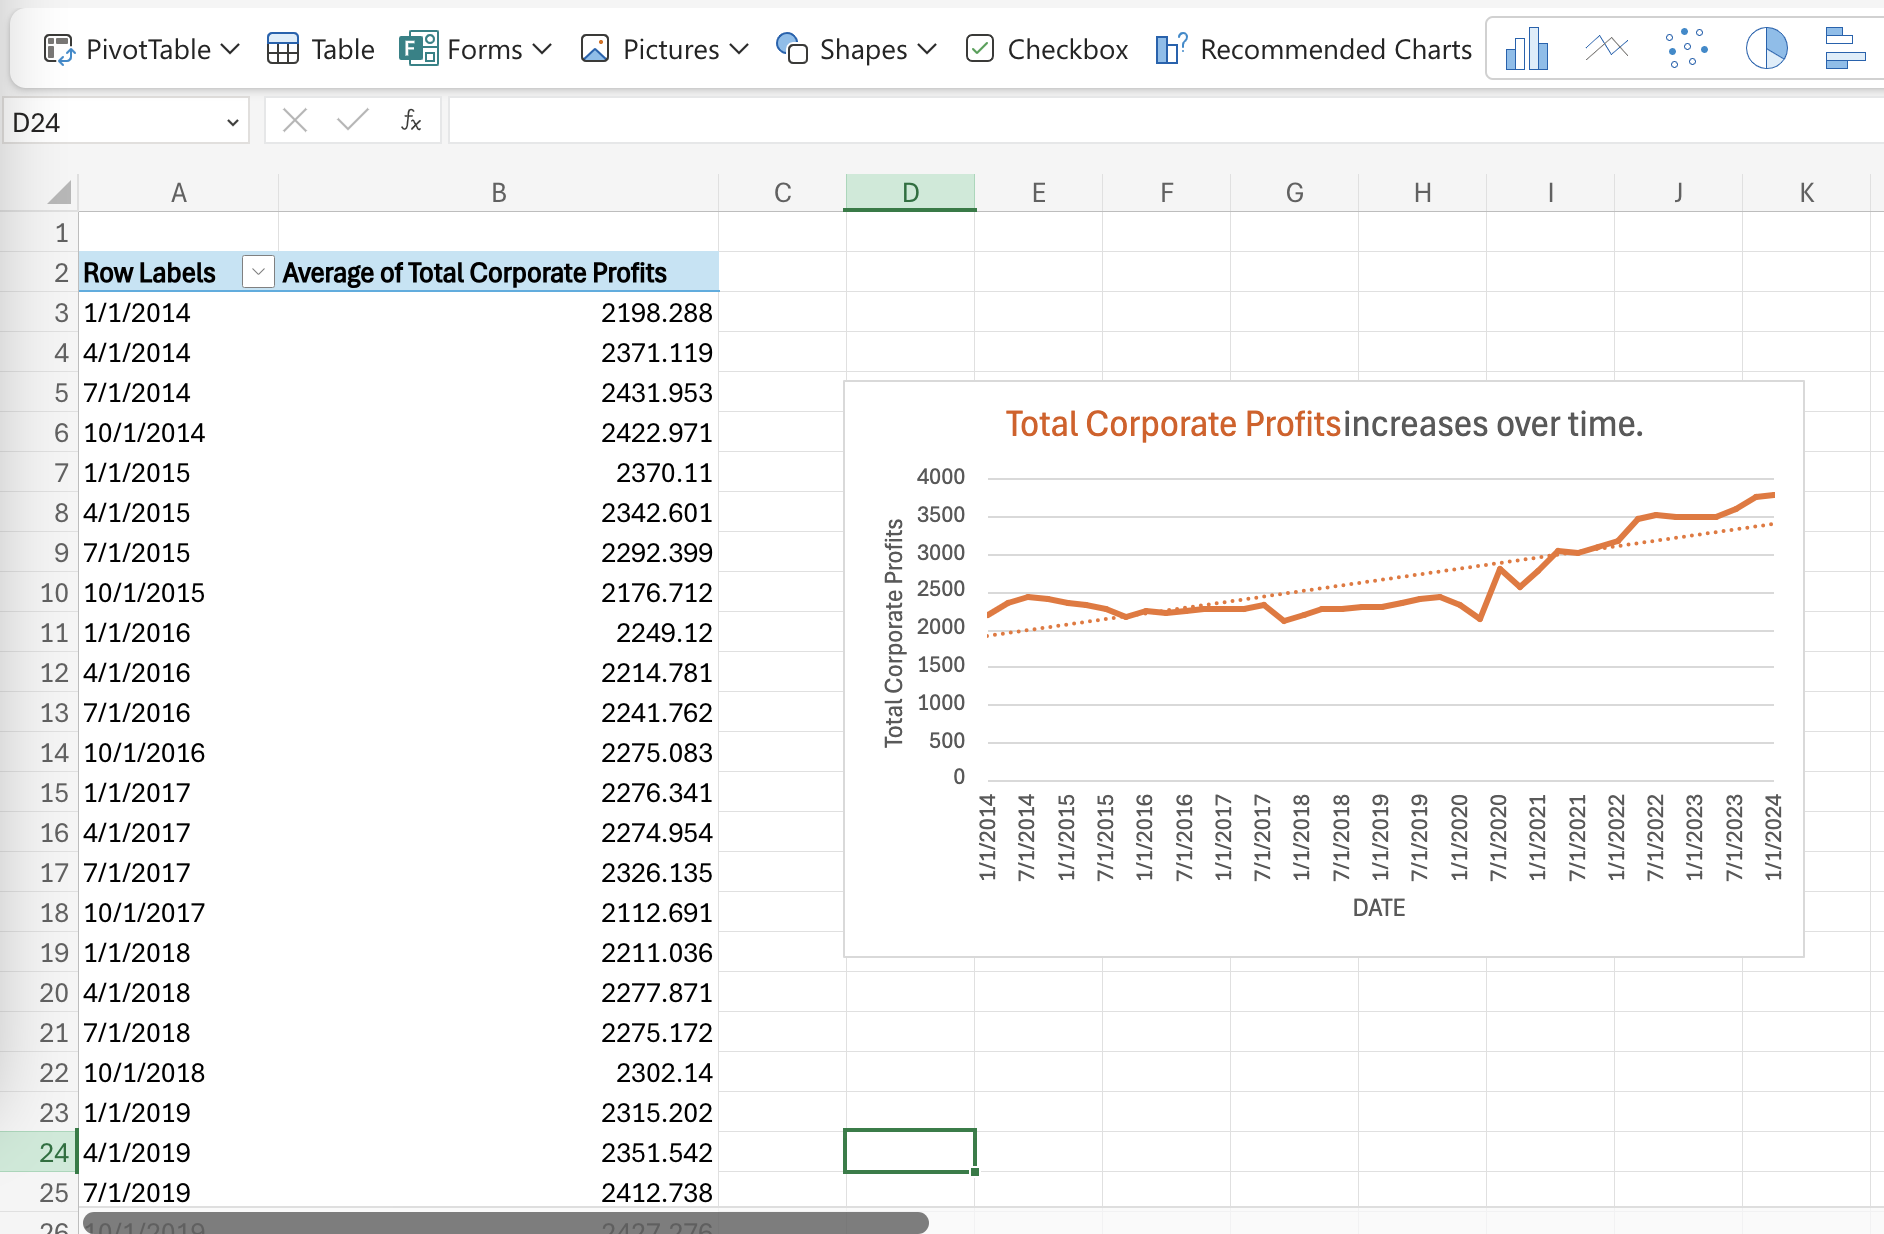
\includegraphics{./Excel_1_Unit/Week1_Janice/Week 1/Week 1 Friday/Average_CP.png}

When I added a graph from the `Recommended Charts', a new sheet is
created along with corporate profits summed into yearly instead of
quarterly.

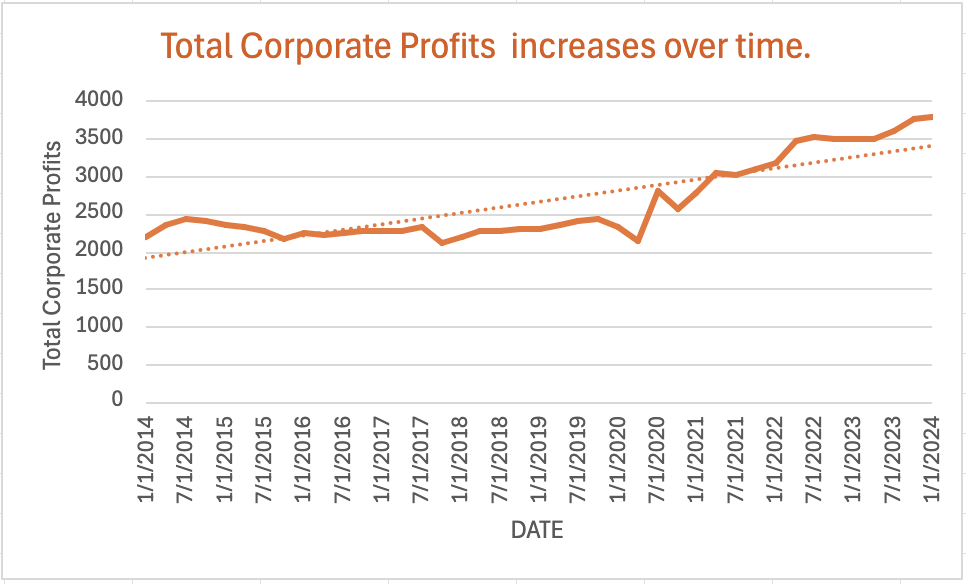
\includegraphics{./Excel_1_Unit/Week1_Janice/Week 1/Week 1 Friday/Linechart.png}

\begin{itemize}
\tightlist
\item
  Total corporate profits increase over the 10 year period.
\item
  There are some significant declines in corporate profits The two major
  declines occurred in the span of end of quarter of 2019 to end of
  quarter of 2020. in the late quarter of 2019 to 2020. It is evident
  that the COVID-19 pandemic caused the sudden drop in corporate
  profits, with the lock-down, inflation, and slowdown of the economy.
  The economy healed in the first two quarters of 2020 as the lock-downs
  are alleviated, however declined again in the end of quarter of 2020.
\item
  The private enterprises' profits appear to be very steadily increasing
  from first quarter of 2022 to the first quarter of 2024. The total
  corporate profits appear to be higher than the average total corporate
  profits dotted line, signifying that the increase in total corporate
  profits are quite significant.
\end{itemize}

\subsubsection{Scatterplot 1: Domestic Industries (Non-financial:
Manufacturing)
vs.~Federal}\label{scatterplot-1-domestic-industries-non-financial-manufacturing-vs.-federal}

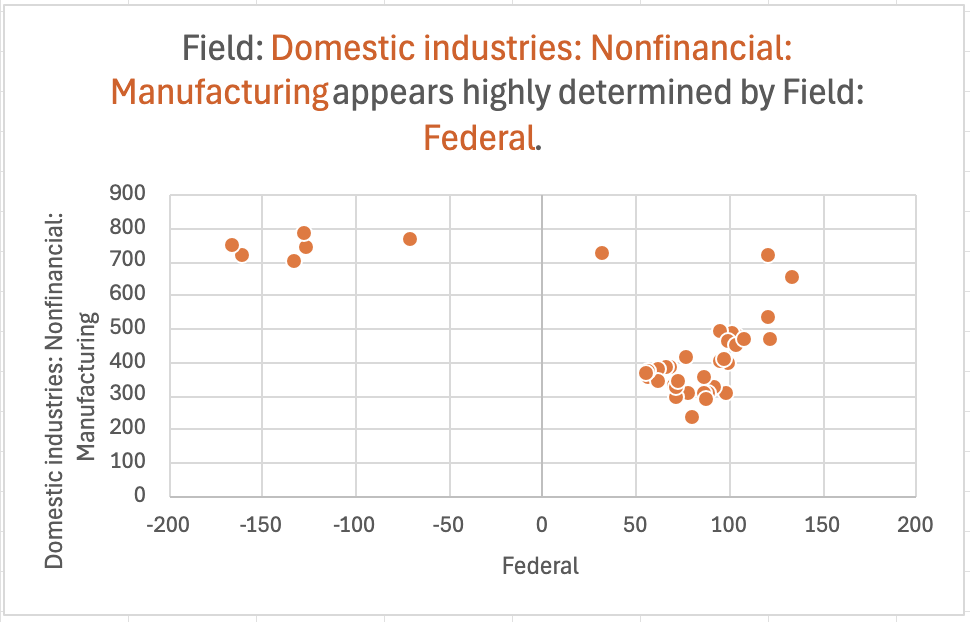
\includegraphics{./Excel_1_Unit/Week1_Janice/Week 1/Week 1 Friday/Scatterplot1.png}

\begin{itemize}
\tightlist
\item
  ``Domestic Industries: Non-financial: Manufacturing'' appears to have
  an inverse relationship with ``Federal''
\end{itemize}

As `Manufacturing' is high at a range of 675-825 billion dollars,
`Federal' appears to be on hundreds of billion dollars loss. However, as
`Manufacturing' decreases to below 600 billion dollars, `Federal's'
corporate profits improved to a range of 50-125 billion dollars.

\subsubsection{Scatterplot 2: Wholesale trade vs.~Transportation and
warehousing}\label{scatterplot-2-wholesale-trade-vs.-transportation-and-warehousing}

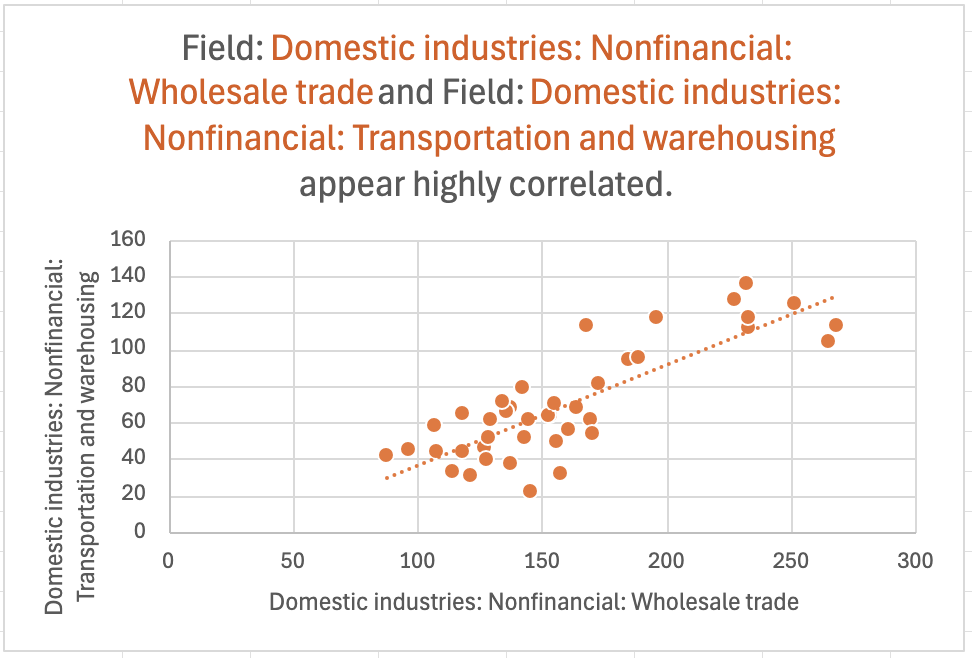
\includegraphics{./Excel_1_Unit/Week1_Janice/Week 1/Week 1 Friday/Scatterplot2.png}

\begin{itemize}
\tightlist
\item
  As wholesale trade's corporate profits increases, the corporate
  profits in the sub-sector of transportation and warehousing also
  increases.
\end{itemize}

The direct and proportional relationship of the two sub-sectors make
sense, as wholesale trade involves purchasing goods in large quantities
and reselling them in smaller quantities to businesses and other
wholesalers, directly involving transportation and warehousing of the
goods.

\subsubsection{Barchart: Non-financial vs.~Financial Domestic
Industry}\label{barchart-non-financial-vs.-financial-domestic-industry}

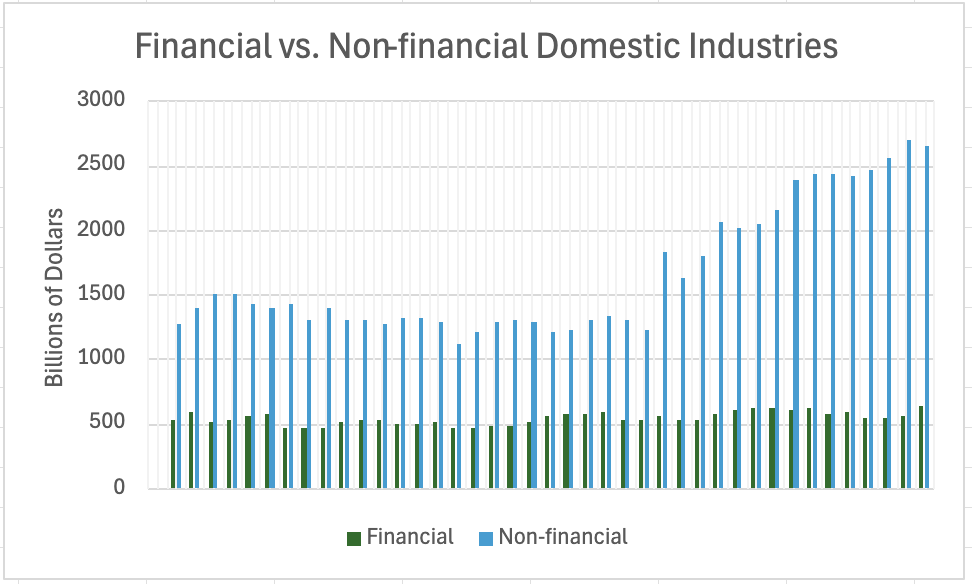
\includegraphics{./Excel_1_Unit/Week1_Janice/Week 1/Week 1 Friday/Barchart.png}

\begin{itemize}
\tightlist
\item
  The non-financial domestic industry's corporate profits are growing
  more significantly compared to the financial domestic industry's
  stable corporate profits
\end{itemize}

The non-financial domestic industry are growing more rapidly, especially
in the last half of the decade. The financial domestic industry has over
2500 billions of dollars of corporate profits in the first quarter of
2024. Meanwhile, the financial domestic industry appears to have stable
corporate profits throughout the past 10 years, as its corporate profits
are varying slightly from year to year and are stuck under 750 billion
dollars.

\subsubsection{Piechart: Non-financial makes up the majority of the
domestic industry's corporate
profits}\label{piechart-non-financial-makes-up-the-majority-of-the-domestic-industrys-corporate-profits}

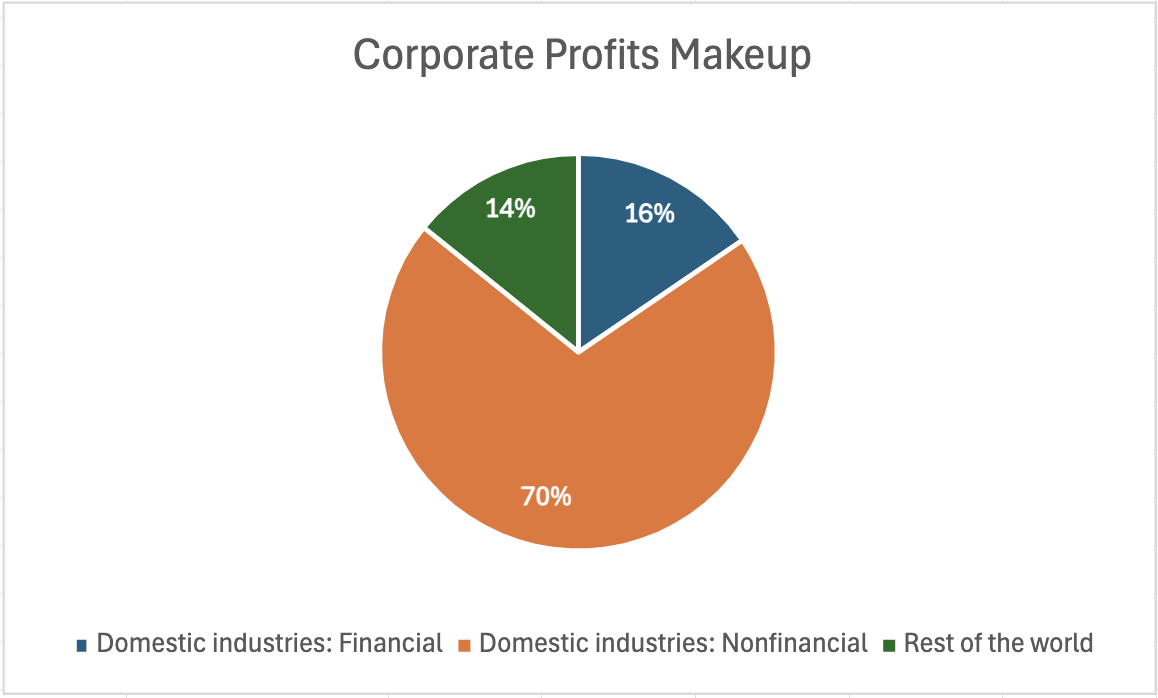
\includegraphics{./Excel_1_Unit/Week1_Janice/Week 1/Week 1 Friday/Piechart.png}

\begin{itemize}
\tightlist
\item
  Non-financial domestic industry takes 70\% of the domestic industry's
  corporate profits, while the rest of the world takes up only 14\% of
  the domestic industry's corporate profits.
\item
  As stated in a study, non-financial corporations are responsible for a
  large share of the economic activity in most advanced economies
  (Tebrake \& O'hagan, n.d.), which maakes sense as a lot of the
  important sub-sectors belong to the non-financial industry (including
  manufacturing of durable and non-durable goods, wholesale trade,
  retail trade, utilities, and information)
\end{itemize}

\subsection{References}\label{references}

\begin{itemize}
\item
  Tebrake, J., \& O'hagan, P. (n.d.). Understanding Financial Accounts
  The financing of non-financial corporations. Retrieved August 31,
  2024, from
  \url{https://www.oecd-ilibrary.org/docserver/9789264281288-8-en.pdf?expires=1725145368&id=id&accname=guest&checksum=CE2ED779ABF58E8BEB69C041927BC309}
\item
  \url{https://fred.stlouisfed.org/}.
\item
  \url{https://fredaccount.stlouisfed.org/public/datalist/6257}
\end{itemize}

\bookmarksetup{startatroot}

\chapter{National Center for Education Statistics - Chris
Jacob}\label{national-center-for-education-statistics---chris-jacob}

\section{Wednesday}\label{wednesday-3}

\subsection{Diamonds Dataset}\label{diamonds-dataset}

I applied the learnings and findings from the Excel Unit to another
dataset, the diamonds\_ggplot2.csv set. -
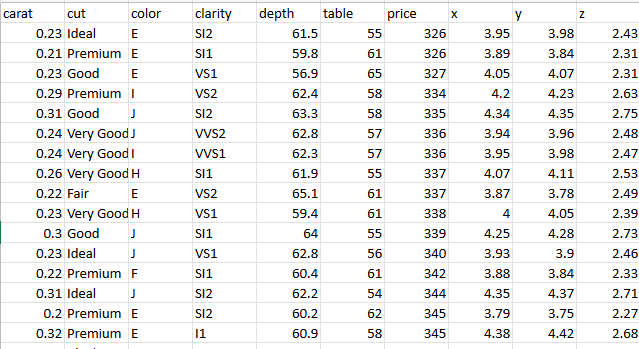
\includegraphics{./Excel_1_Unit/Week1_Chris/VIZ_step1.png} - The
Diamonds dataset defines the different characteristics of a diamond
namely, carat, cut, color, clarity, depth, price, and lengths in the x,
y, and z direction The dataset itself did not have any NA values, and
hence did not need any additional steps for cleaning the data. An
interesting observation to be made was that there are several
interesting correlations between the columns that can help us observe
some basic trends in the diamond trading business. There were more than
53,000 records collected, and so this dataset is very comprehensive!

\subsubsection{Preparing the dataset}\label{preparing-the-dataset}

Considering the size of the dataset, I had to use 500 random records to
create my visualizations. Here's a step by step guide on how I did that.

\paragraph{Add a random number column}\label{add-a-random-number-column}

\begin{itemize}
\tightlist
\item
  Choose a column and add the RAND() function to the column. Double
  click on the bottom right of the cell to paste the function to the
  rest of the rows in the dataset. This creates a random number between
  0 and 1.
  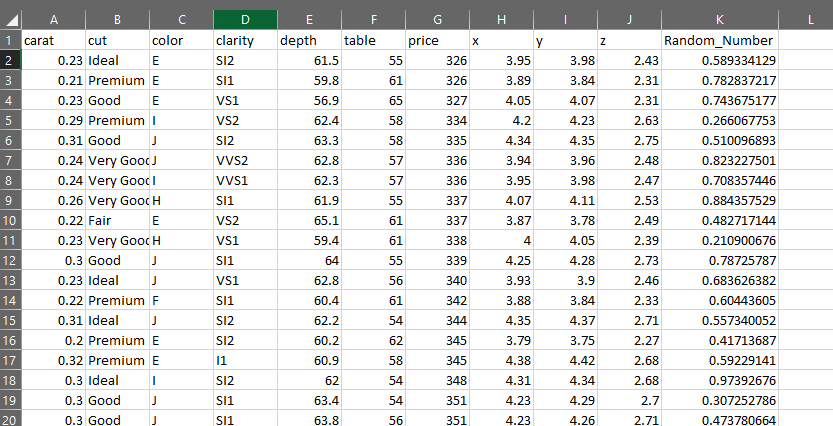
\includegraphics{./Excel_1_Unit/Week1_Chris/random_number_column.png}
\item
  Next, we apply a filter to the entire dataset, and use the random
  number column (sorting it from smallest to largest). This
  automatically rearranges the data records, making the first 500
  random.
  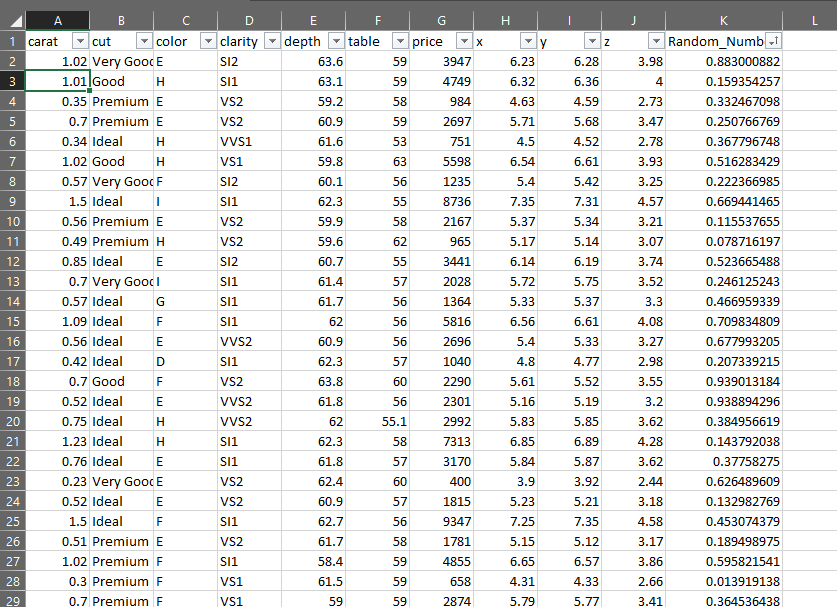
\includegraphics{./Excel_Unit_1/Week1_Chris/filter_for_randomness.png}
\item
  Copy the first 500 records to a new sheet. This now becomes your 500
  records that give you a true random overview of the Diamonds dataset.
  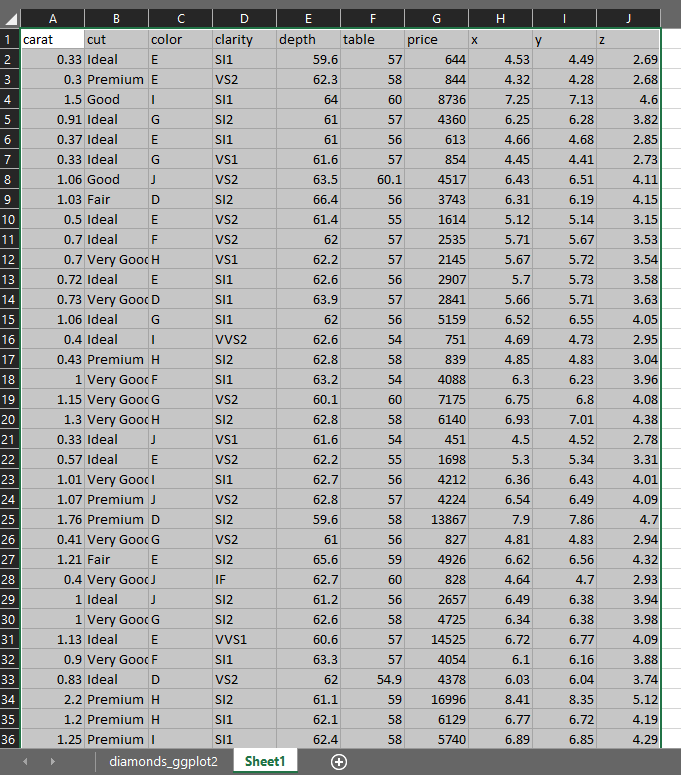
\includegraphics{./Excel_Unit_1/Week1_Chris/new_sheet_with_random_values.png}
\item
  Since the records didn't contain any NA values, this looked like the
  only preparation I needed to do.
\end{itemize}

\paragraph{Creating visualizations}\label{creating-visualizations}

\subparagraph{Scatter Plot: Carat VS
Price}\label{scatter-plot-carat-vs-price}

\begin{itemize}
\tightlist
\item
  The first plot I created was a scatter plot that visualized the
  relationship between the carat of the diamond and the price it would
  sell at
  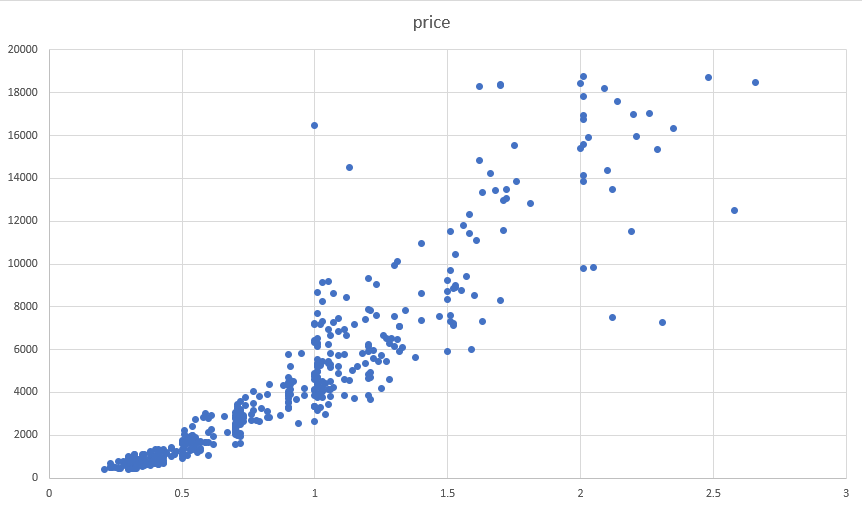
\includegraphics{./Excel_1_Unit/Week1_Chris/scatter_carat_vs_price.png}
\item
  From this, we can see that the dimaonds that have a higher carat sell
  for more.
\end{itemize}

\subparagraph{Histogram: Sum of Price by
Color}\label{histogram-sum-of-price-by-color}

\begin{itemize}
\item
  The next plot I created was a histogram that visualized the
  relationship between the prices and the color of the diamond.
  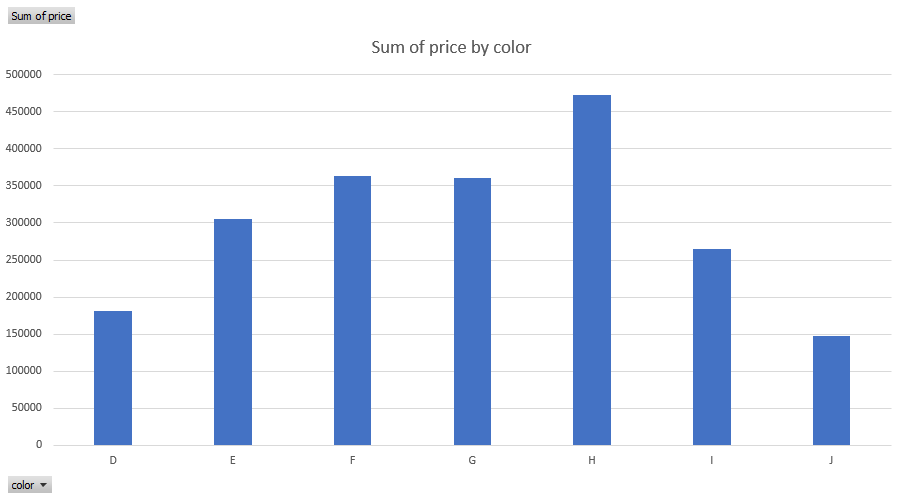
\includegraphics{./Excel_1_Unit/Week1_Chris/histogram_price_color.png}
\item
  From this chart, it was clear to see that the diamonds that had the
  most value were those with the `H' coloration.
\end{itemize}

\subparagraph{Other charts}\label{other-charts}

\begin{itemize}
\tightlist
\item
  When trying to create more visualizations, I observed that not all
  charts were capable of visualizing this data, and furthermore, given
  the size of the dataset, all operations were much slower on the online
  excel sheet.
\item
  I believe the best visualization for such data is the Scatter Plot of
  Price vs Carats, because it captures the inherent reality that more
  carats means more price. All in all, it was an interesting start to
  the class and helped me better understand how visualizations can be
  achieved on excel.
\end{itemize}

\section{Friday}\label{friday-3}

\subsection{NCES Education Dataset}\label{nces-education-dataset}

NCES Education Dataset is extremely vast and includes several different
studies conducted over a range of years. Today, we'll only be focusing
the High School Longitudinal Study of 2009.
\url{https://nces.ed.gov/surveys/hsls09/index.asp}

The High School Longitudinal Study of 2009 (HSLS:09) is a comprehensive
study conducted by the National Center for Education Statistics (NCES).
It tracks a cohort of students who began 9th grade in 2009, following
them through their high school years and beyond into postsecondary
education and the workforce. The study focuses on students' educational
trajectories, especially in STEM, examining factors like course-taking
patterns, college aspirations, and career choices. The data collected
provides insights into how high school experiences influence long-term
educational and career outcomes.

\subsubsection{Working with the datset}\label{working-with-the-datset}

\begin{itemize}
\tightlist
\item
  This can be an extremely complicated process. The first step should be
  to go to \url{https://nces.ed.gov/datalab/membership/register} and
  registering yourself to access all the benefits that NCES datalabs
  offer.
  \includegraphics{./Excel_1_Unit/Week1_Chris/register_new_user_chris.png}
\item
  This gives us access to the data lab dashboard. Since we can't use
  excel because of the extremely large size, so we'll have to use the
  datalabs power stats tool for this.
  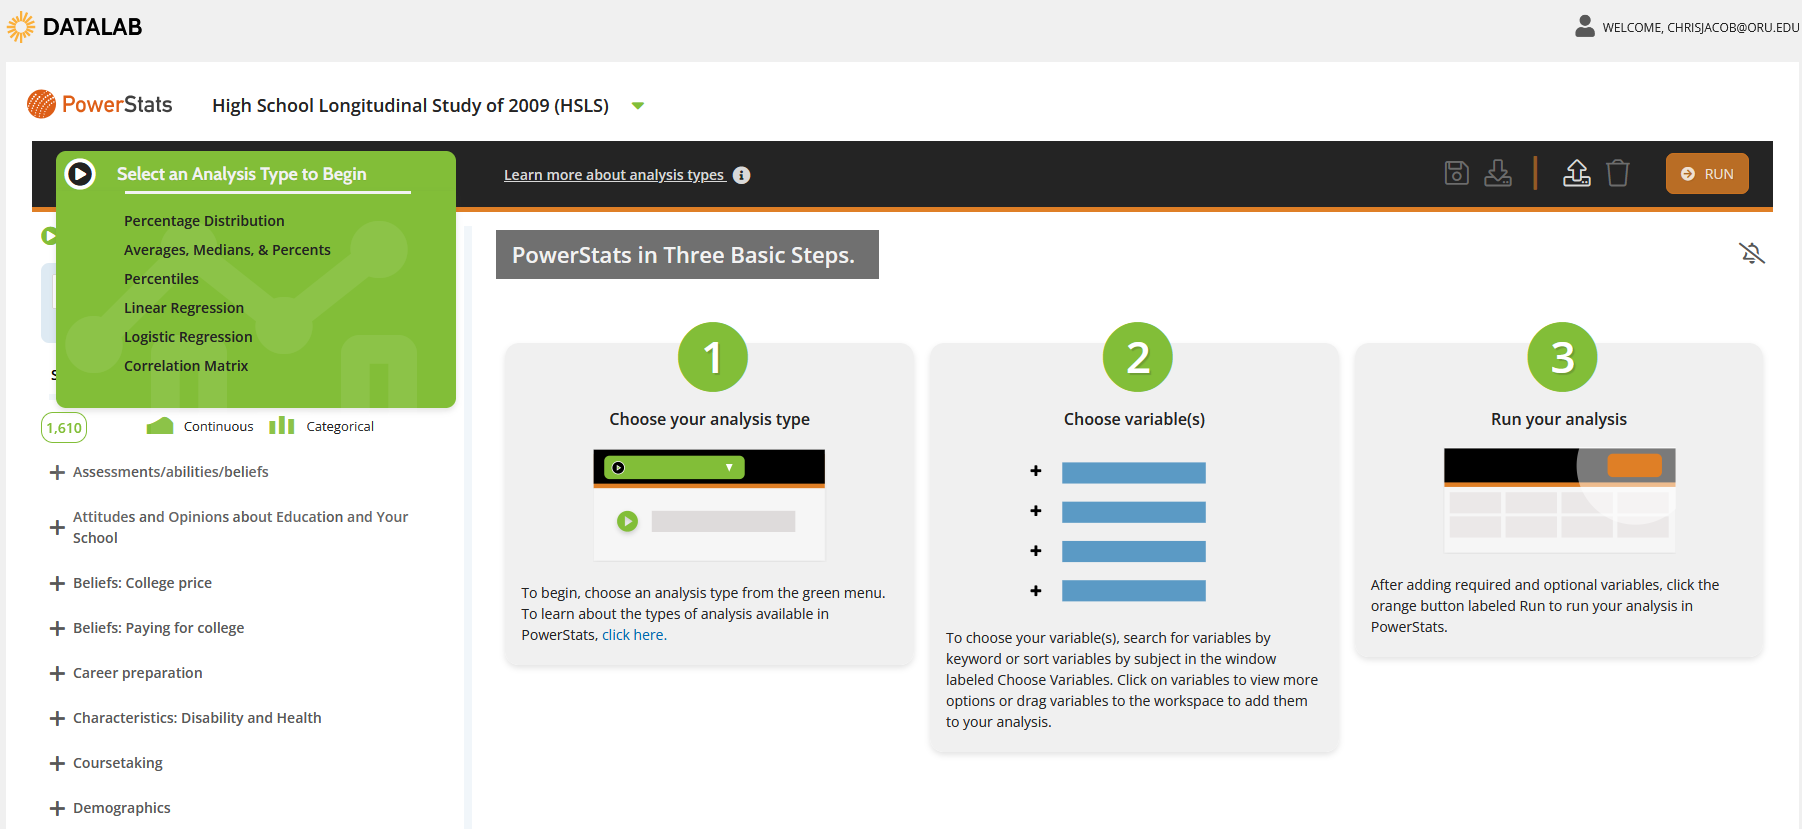
\includegraphics{./Excel_1_Unit/Week1_Chris/datalabs_overview.png}
\end{itemize}

\subsubsection{Simple Visualization}\label{simple-visualization}

\begin{itemize}
\item
  Considering that I couldn't use excel for this process, it was
  interesting to see the amount of data and variables I had at my
  disposal for this project. For example, just the keyword `STEM' has
  294 variables attached to it.
\item
  One comparison I made using the PowerStats tool to create a percentage
  analysis of the relationship between variables S1 and S3.

  \begin{itemize}
  \tightlist
  \item
    S1 looks into how math teachers make math so easy to understand.
    This is divided as `Strongly Agree', `Agree', `Neutral', `Disagree',
    `Strongly Disagree'
  \item
    S3 shows how students might consider STEM as a major.
  \end{itemize}
\item
  This visualization further strengthens the premise that teachers are
  the defining factors in a lot of the future decisions that students
  make.
\end{itemize}

\begin{figure}[H]

{\centering 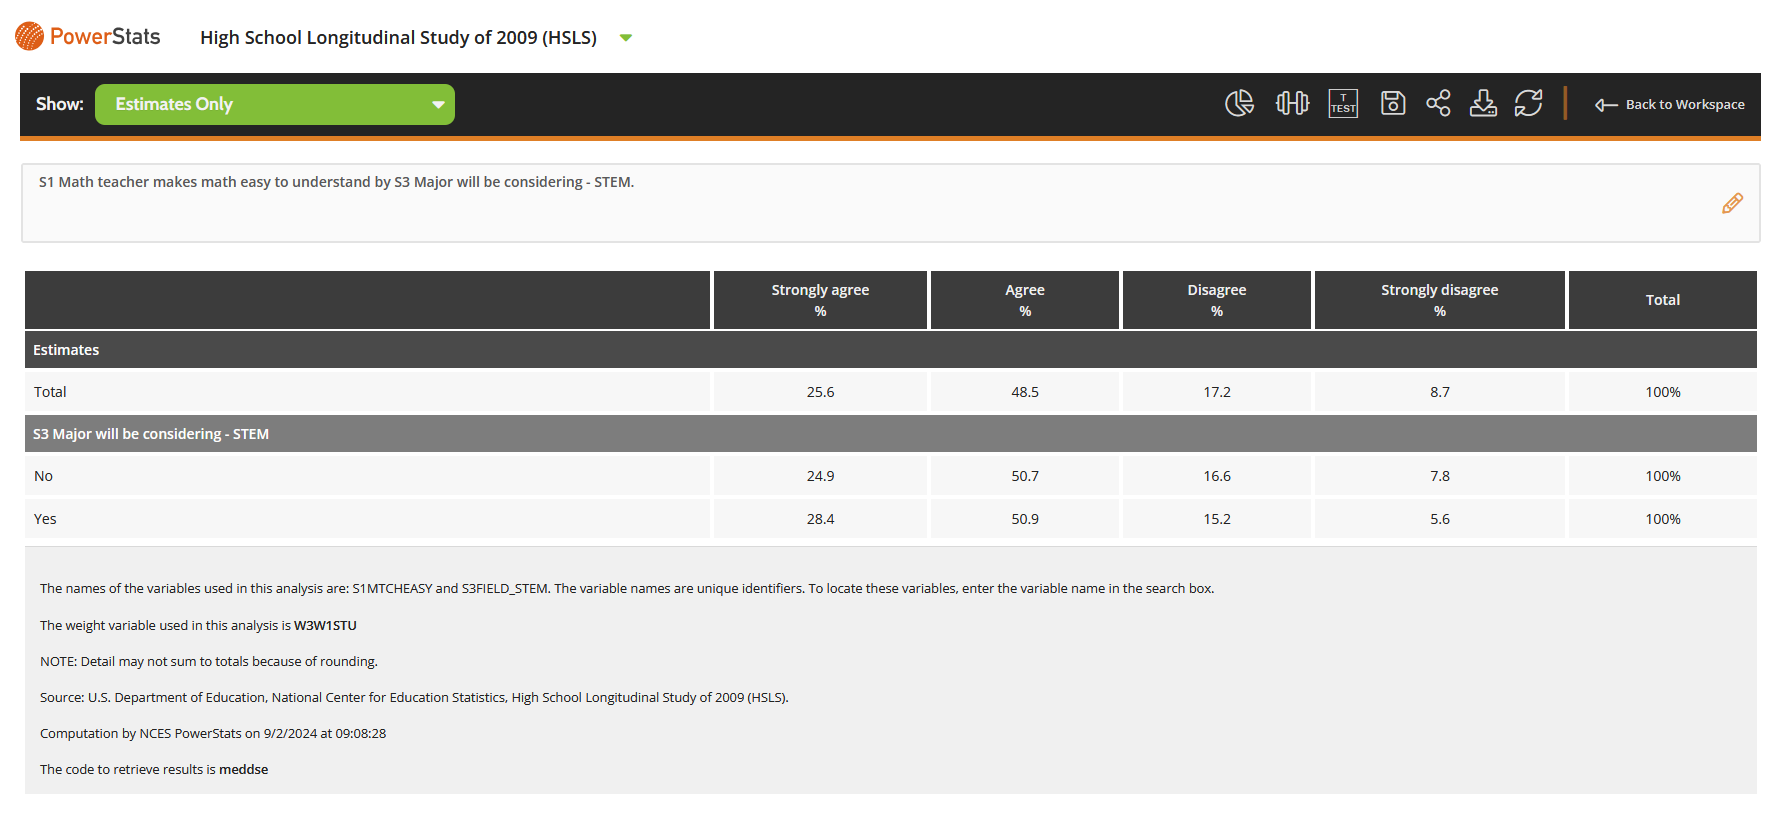
\includegraphics{./Excel_1_Unit/Week1_Chris/stem_math_visualization.png}

}

\caption{Pecentage Analysis}

\end{figure}%

\begin{itemize}
\tightlist
\item
  It further allowed me to use the bar chart to show this information
  visually.
  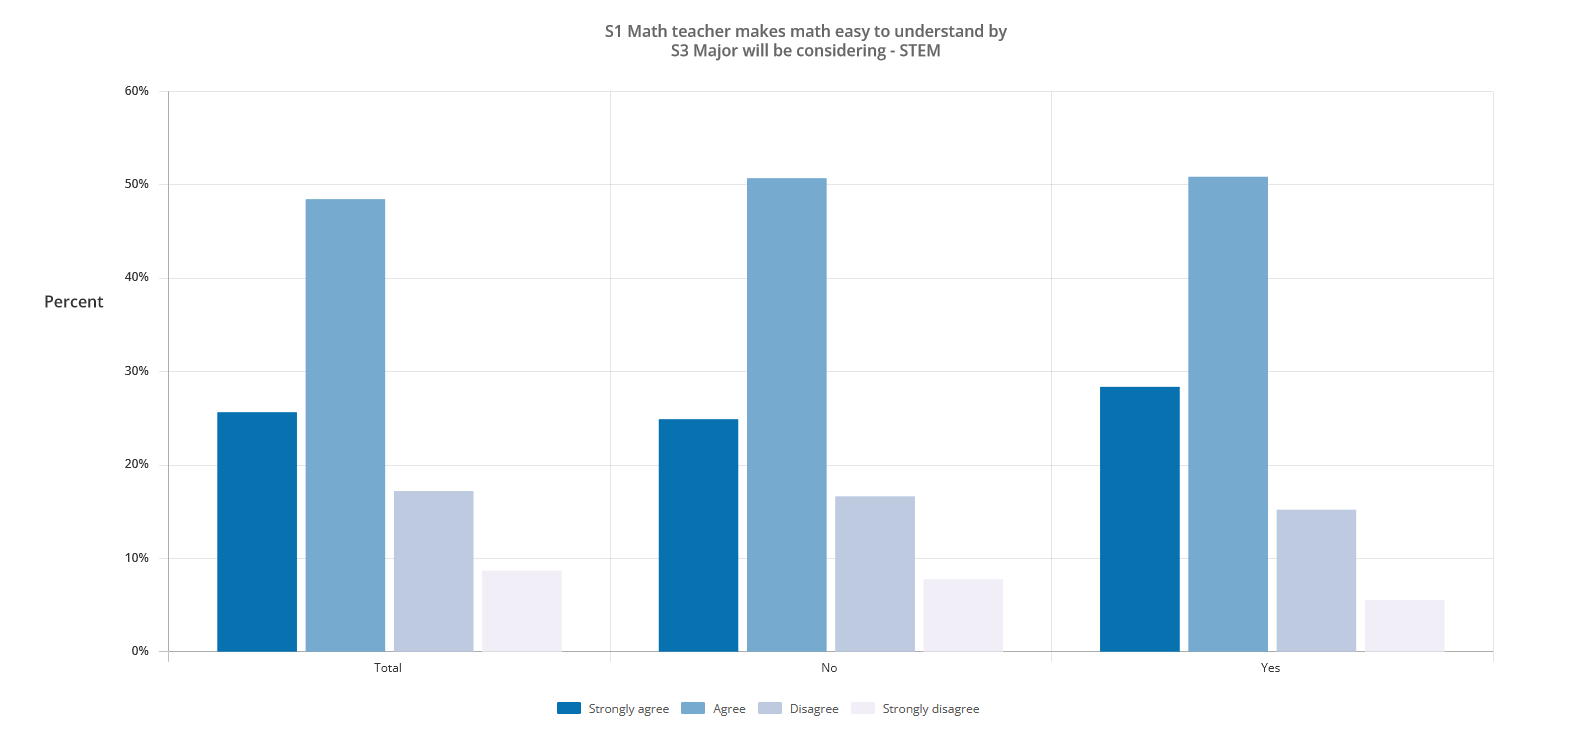
\includegraphics{./Excel_1_Unit/Week1_Chris/stem_math_chart.png}
\end{itemize}

\subsubsection{Inference}\label{inference}

\begin{itemize}
\tightlist
\item
  These visualizations make it clear that teachers who help make
  concepts like math and science easier to understand, help these
  students choose STEM as a major in university.
\item
  This insight will further add to the `STEM Focused' dataset that I'll
  be building during this semester.
\end{itemize}

\subsection{Conclusion}\label{conclusion}

\begin{itemize}
\tightlist
\item
  Given the vastness of this dataset, I believe it's important for me to
  better understand and comprehend this dataset, so that I can fully
  utilize and appreciate all the data collected. Although I wasn't able
  to use Excel on this dataset, the skills learned in the previous
  classes definitely helped set me up for success with this.
\end{itemize}




\end{document}
